\chapter{Diseño} \label{disenio}
En este cuarto capítulo se establecerá la estructura de la plataforma, no sólo a nivel técnico, sino también a nivel visual. Primeramente se definirá la arquitectura que presentará la plataforma, explicando cada uno de los elementos que la conforman, base de datos, servidor y cliente. Para ello, tanto en el servidor, como en el cliente se expondrán dos diagramas UML de paquetes diseñados siguiendo las indicaciones del artículo \textit{''An Overview of Structural
UML Diagrams''}\cite{bhatt2021overview}.

\section{Arquitectura MEAN}
\begin{figure}[H]
    \centering{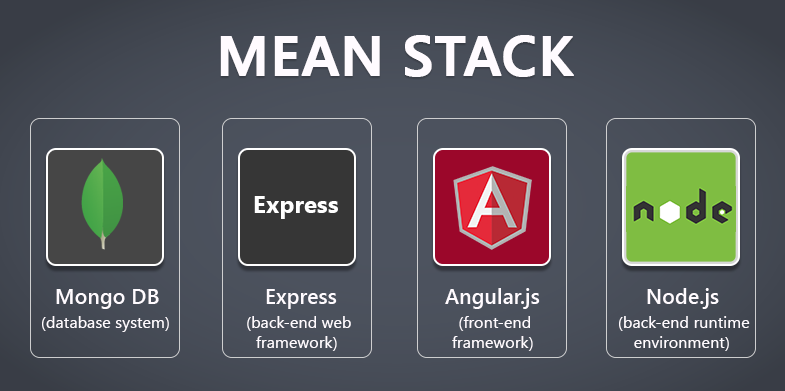
\includegraphics[scale=0.4]{doc/imagenes/mean.png}}
    \caption{Stack MEAN (Mongo, Express, Angular y Node)}
    \label{mean}
\end{figure}

Para la arquitectura del proyecto se ha optado por hacer uso del stack software MEAN \cite{nirgudkar2017mean} (Figura \ref{mean}), acrónimo que hace referencia a las tecnologías que lo conforman: MongoDB, Express.js, Angular y Node.js. 

\begin{figure}[H]
    \centering{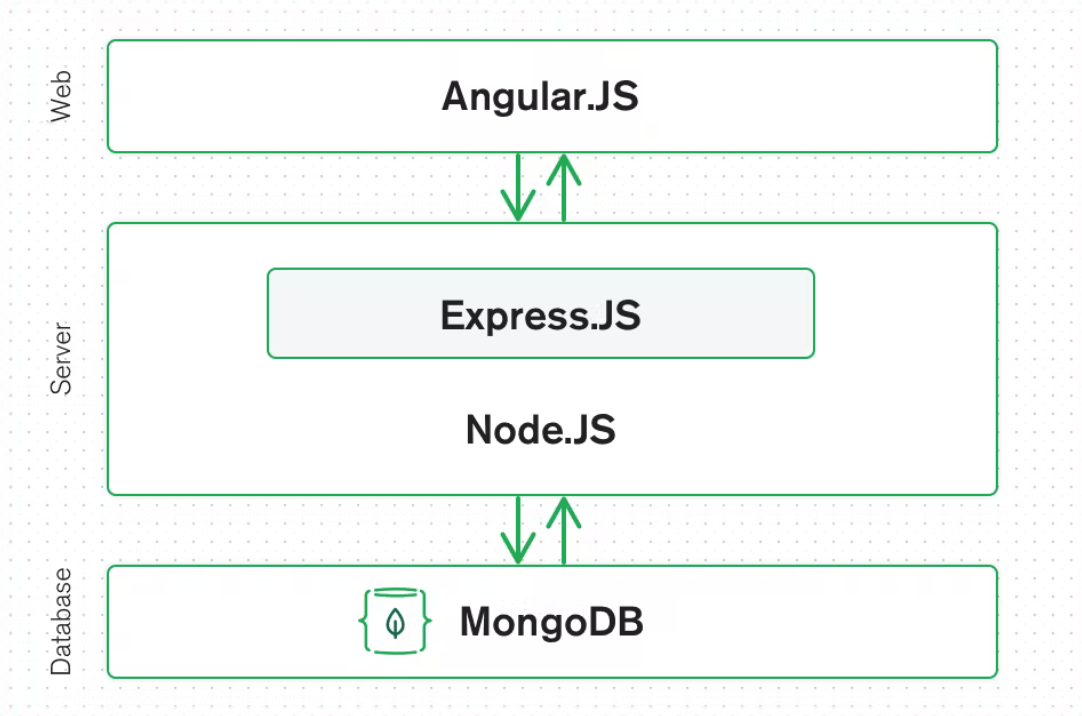
\includegraphics[scale=0.25]{doc/imagenes/mean-architecture.png}}
    \caption{Arquitectura en capas de MEAN}
    \label{mean-architecture}
\end{figure}

Se trata de un stack software basado en JavaScript para el desarrollo de aplicaciones web, cuyo diseño hace una división en capas de la parte del cliente, el servidor y la base de datos (Figura \ref{mean-architecture}). \bigskip

Se ha decidido aplicar este stack en concreto a la arquitectura del proyecto por varios motivos. El primero es que, a pesar de que la desarrolladora no había trabajado anteriormente con las tecnologías Express.js y Node.js, sí que lo había hecho con Angular y MongoDB, por lo que esa falta de experiencia en el desarrollo de la parte del servidor es compensada. Otro de los motivos a mencionar es que MEAN es de código abierto, y en consecuencia no sólo abarata el coste del proyecto, sino que también significa que la documentación de la que se dispone sea considerablemente extensa debido su gran comunidad de soporte. Por supuesto, un punto muy positivo que presenta MEAN, tal y como afirma Bakwa D. Dunka et al. \cite{dunka2018simplifying}, es el uso de JavaScript en la capa del servidor y del cliente, lo cual conlleva mayor simplicidad en la implementación y no se necesita aprender un nuevo lenguaje. Asimismo, otra característica realmente positiva a mencionar es la complicidad que existe entre sus tecnologías, pues, como se comentará más adelante, en la parte del cliente se va a utilizar el componente Angular Schedule de Syncfusion \footnote{\url{https://ej2.syncfusion.com/angular/documentation/schedule/getting-started/}}, el cual se trata de un componente de Angular que trabaja con datos de tipo JSON para las citas. En cuanto al uso de la base de datos no relacional con MongoDB, resulta perfecto ya que las citas vendrán acompañadas de descripciones potencialmente largas y sin formato. Por último, resaltar una característica mencionada en el artículo escrito por Sanchit Aggarwal et al. \cite{aggarwal2018comparative}: el buen rendimiento presentado por Angular para manejar un gran número de datos, ya que en cuanto a lo que concierne a este proyecto un calendario en cierto momento llegará a contener cientos de citas.

\subsection{Diseño de la base de datos} \label{bd}

Para el diseño de la base de datos se han planteado las siguientes dos colecciones (Figura \ref{bd}):

\begin{figure}[H]
    \centering{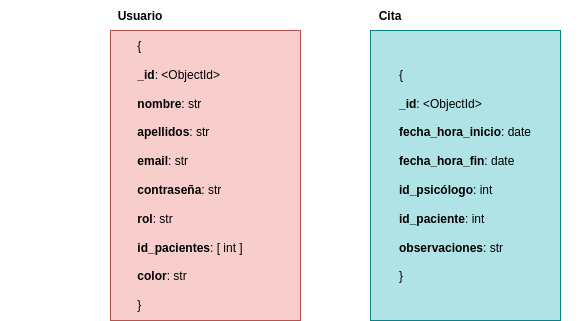
\includegraphics[scale=0.5]{doc/imagenes/bd.png}}
    \caption{Diagrama de la base de datos}
    \label{bd}
\end{figure}

La base de datos consta de dos colecciones: \textbf{Usuario} y \textbf{Cita}. La primera contiene el id del usuario, nombre, apellido, email, contraseña encriptada y rol del éste en la plataforma (administrador, paciente o psicólogo). Además de estos campos el rol de psicólogo posee un array de ids de pacientes y un color asignado para las citas, si no se poseyera este rol ambos campos serian nulos en el documento. Por otro lado, la colección de Cita contiene el id de la cita, la fecha y hora de inicio y fin de ésta, un campo para posibles observaciones y los ids del paciente y psicólogo de este.

\subsection{Diseño del servidor}

\subsubsection*{Diagrama de paquetes }
En el diseño del servidor de Node.js Express, se ha divido su funcionamiento en 3 componentes (Figura \ref{fig:paquetes-back}) para modularizar y desacoplar funcionalidades: los controladores, los modelos y las rutas. Los controladores serán los encargados de manejar toda la lógica de la aplicación, los modelos represetarán las estructuras de datos de la plataforma y las rutas contendrán los endpoints a los que los usuarios accederan para hacer peticiones a los controladores:

\begin{figure}[H]
    \centering{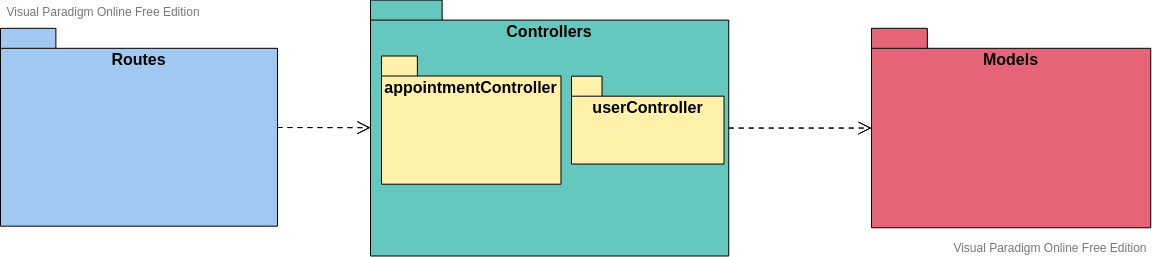
\includegraphics[scale=0.2]{doc/imagenes/package-back.png}}
    \caption{Diagrama de paquetes del backend}
    \label{fig:paquetes-back}
\end{figure}

\subsection{Diseño del cliente}

\subsubsection*{Diagrama de paquetes}
Para el diseño del cliente se ha planteado el siguiente diagrama de paquetes (Figura \ref{fig:paquetes-frontend}) en el que se expone la agrupación de cada componente de Angular en el frontend, donde el componente protagonista es el componente ''main'', el cual en función de la ruta en la que se encuentre el usuario cambiará el componente mostrado.:

\begin{figure}[H]
    \centering{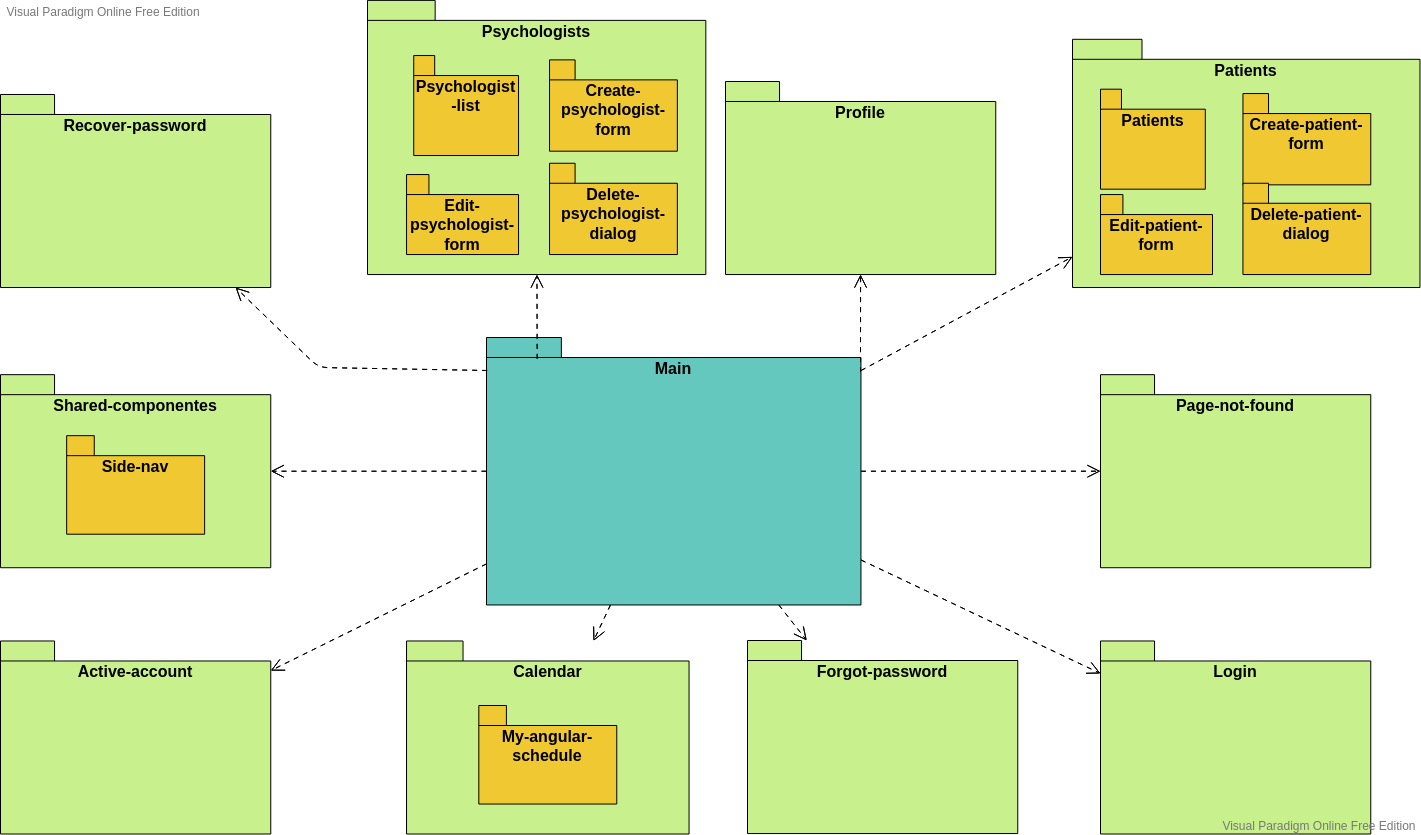
\includegraphics[scale=0.2]{doc/imagenes/diagrama-paquetes-front.png}}
    \caption{Diagrama de paquetes del frontend}
    \label{fig:paquetes-frontend}
\end{figure}

\subsubsection*{Usabilidad y Accesibilidad}
En el diseño de la interfaz de la plataforma se hará uso de Angular Material, siguiendo las guías de diseño proporcionadas por Google Material \footnote{\url{https://material.io/design/guidelines-overview}} para conseguir un diseño, no sólo visualmente estético, sino también usable y accesible proporcionando una experiencia de usuario personalizada. Así lo manifiesta en su libro Venkata Keerti Kotaru \cite{kotaru2020material}, pues la combinación de dicha librería junto con Angular y Typescript generan una poderosa combinación para generar atrativas interfaces de usuario\bigskip

Para el diseño de la interfaz de la plataforma se pretende poner al usuario ante todo, estructurando una web sencilla e intuitiva y evitando todos los puntos negativos comentados en el Capítulo \ref{estado-arte} del Estado del Arte donde se encontraban plataformas con flujos de usuario complejos, poco funcionales. Para ello se ha consultado el libro \textit{''Design Principles in the Development of Dashboards for Business Management''} \cite{martins2022design}. Además, se pretende obtener una interfaz responsiva tanto para tablets como para móviles, siguiendo los consejos de diseño para este tipo de interfaces de Wenjie Li et al. \cite{li2022design}.  \bigskip

Primeramente se debe de definir a qué usuarios se dirige la web. En este caso, los perfiles de usuario a abarcar son numerosos, pues por un lado el personal de la clínica está compuesto por personas con un rango de edad entre 29 y 54 años con conocimientos básicos en la informática y por otro lado el rango de edad de los pacientes es mucho más extenso comprendiéndose, desde jóvenes adolescentes hasta ancianos, por lo que perfectamente habrá casos en los que los conocimientos en informática sean prácticamente nulos. Es por ello que el flujo de usuario debe de ser el más sencillo y directo posible. Siguiendo esta premisa, a continuación se han diseñado los sitemaps que seguirá la plataforma para usuarios identificados y no identificados (Figuras \ref{sitemap-no-identificado} y \ref{sitemap-identificado}), cuyo diseño cumple con las guías que ofrece Google Material para navegación \footnote{\url{https://material.io/design/navigation/understanding-navigation.html}} donde se distinguen tres tipos: navegación hacia adelante, reversa y lateral.

\begin{figure}[H]
    \centering{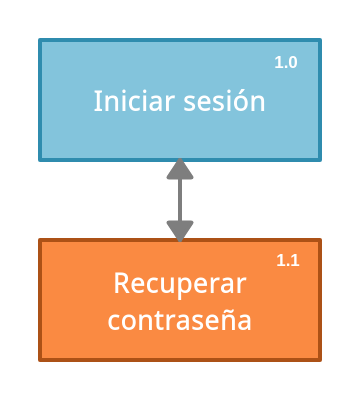
\includegraphics[scale=0.15]{doc/imagenes/sitemap-user-no-registered.png}}
    \caption{Sitemap para un usuario no identificado}
    \label{sitemap-no-identificado}
\end{figure}

\begin{figure}[H]
    \centering{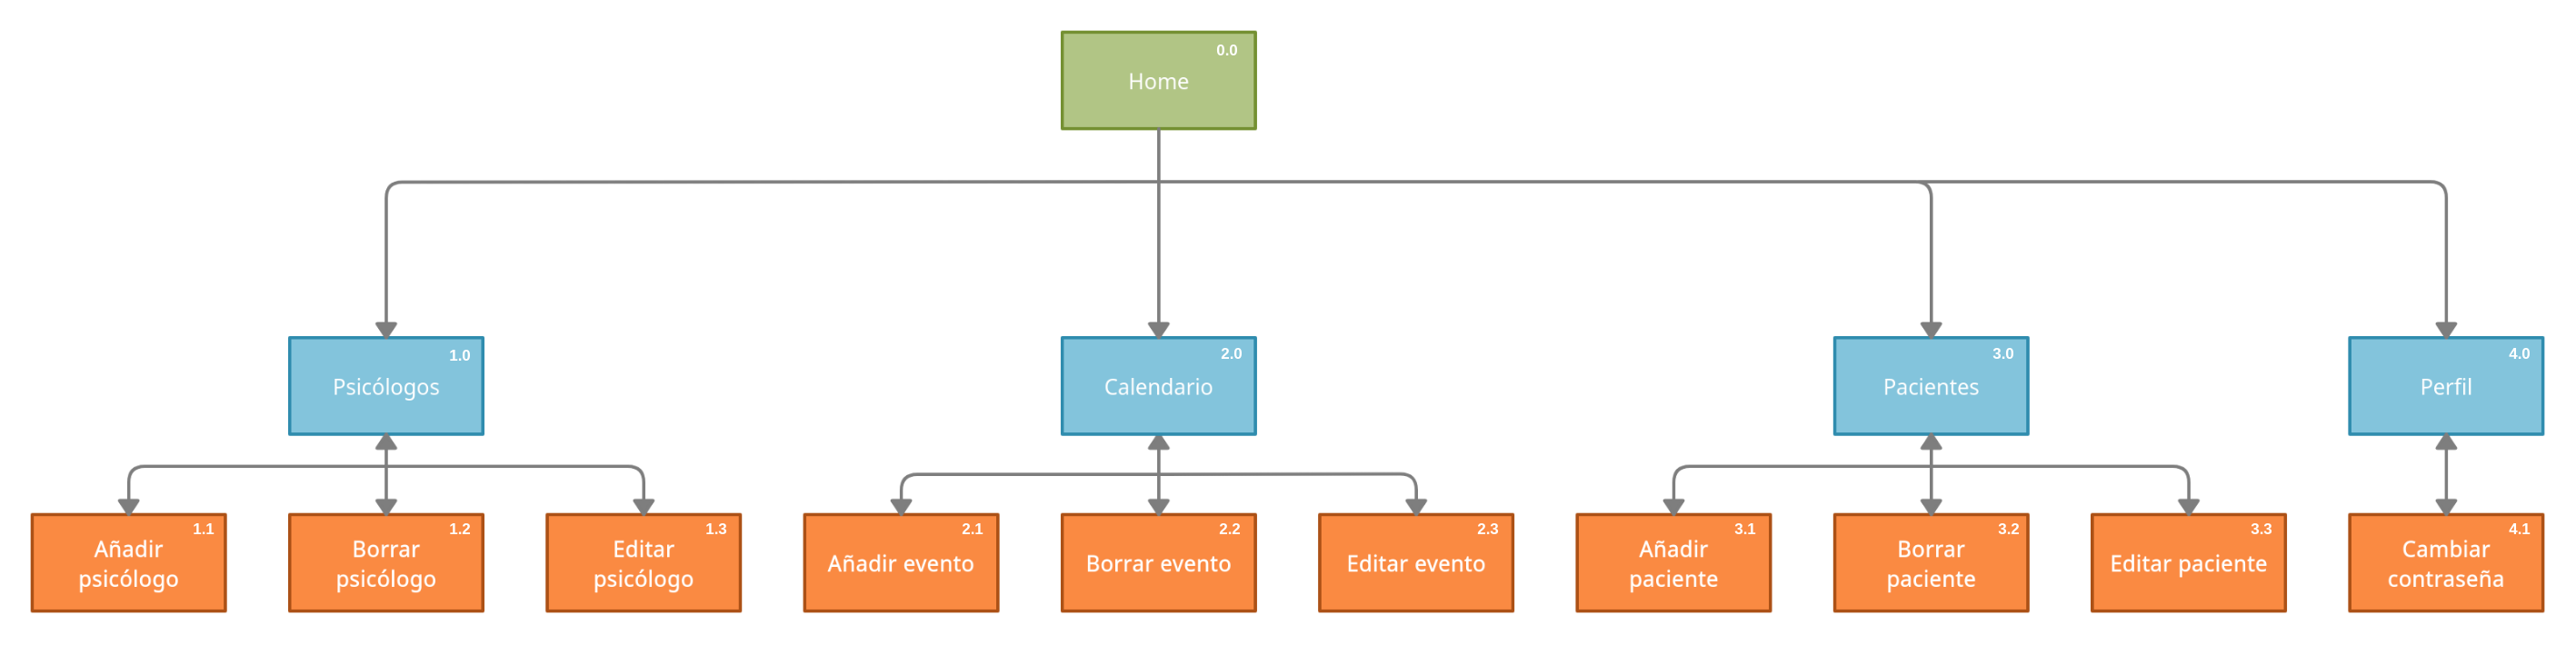
\includegraphics[scale=0.15]{doc/imagenes/sitemap-user-registrado.png}}
    \caption{Sitemap para un usuario identificado}
    \label{sitemap-identificado}
\end{figure}

Ahora que se ha definido la estructura de la página se puede definir el flujo que seguirán sus usuarios. En la definición de dichos flujos se ha pretendido que el usuario no encuentre dificultad alguna en la interacción con la plataforma. Para ello, el flujo seguido para las operaciones CRUD de citas, psicólogos y pacientes es, en esencia, el mismo (Figuras \ref{flow-calendario}, \ref{flow-pacientes} y \ref{flow-psicologos}). La diferencia es la entidad con la que se esta trabajando y el campo ''color'' de los psicólogos que no tienen los pacientes y el campo ''psicólogo'' que no tienen los psicólogos.

\begin{figure}[H]
    \centering{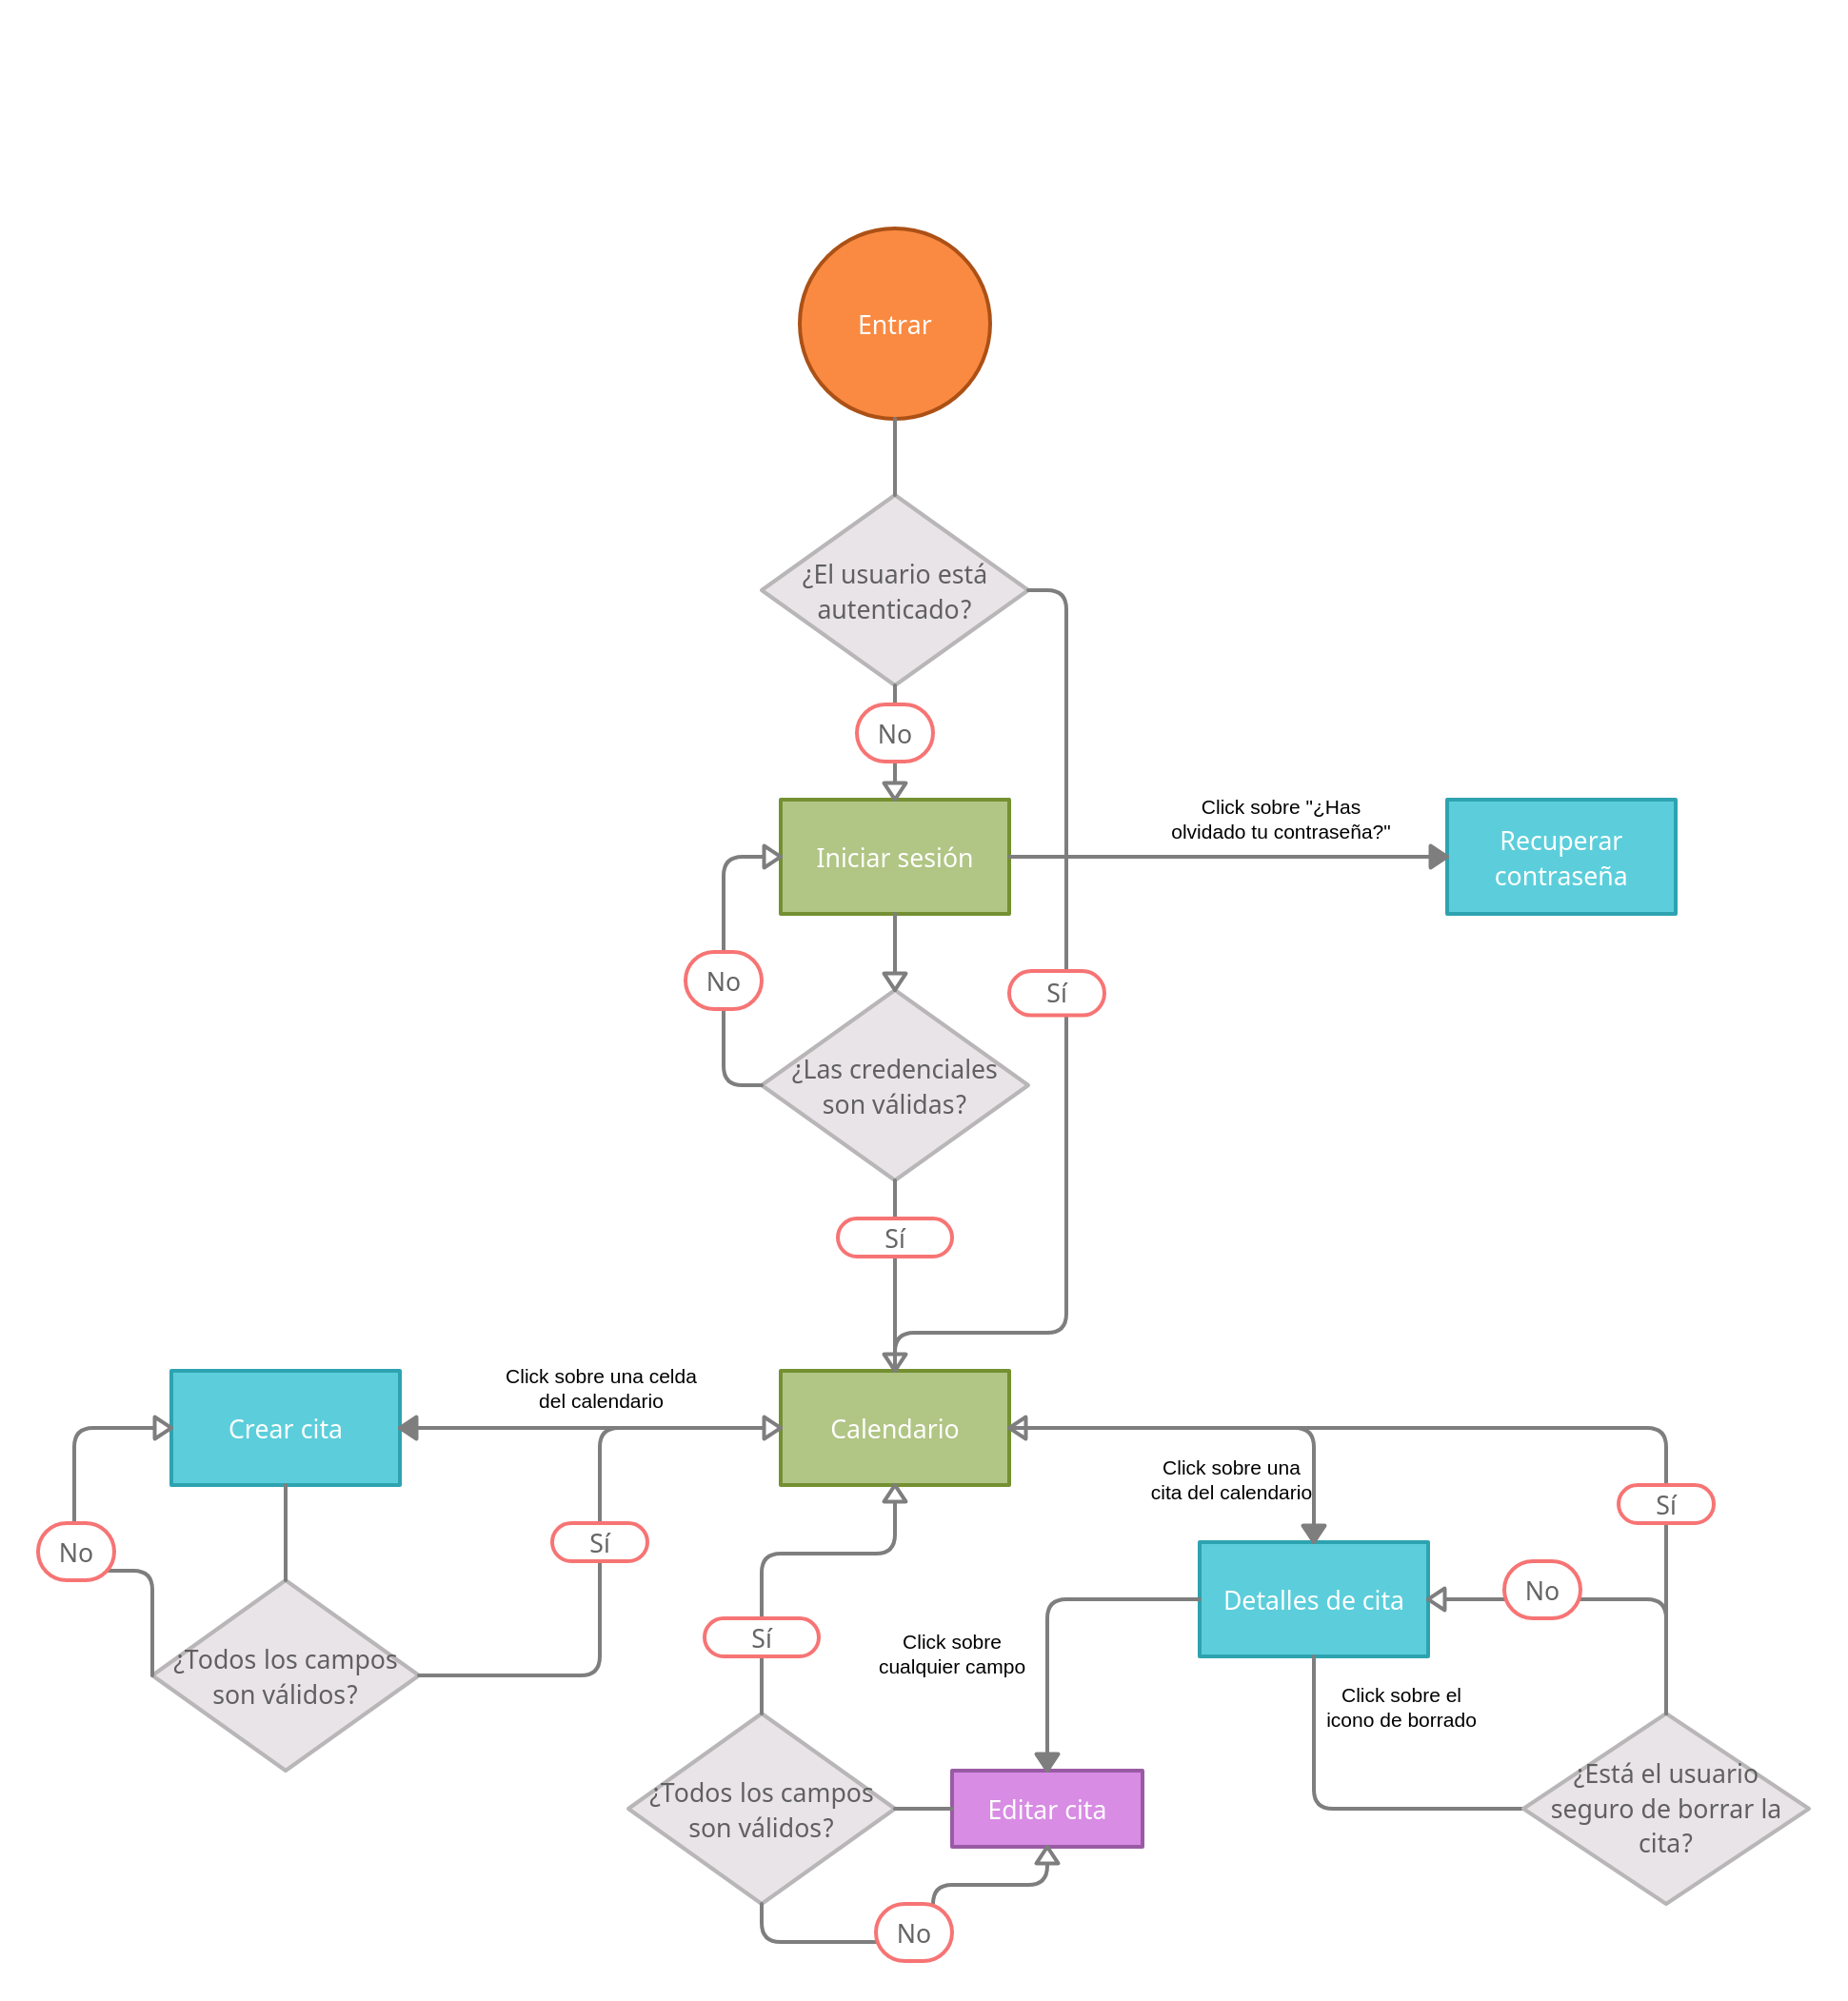
\includegraphics[scale=0.1]{doc/imagenes/flow-calendario.png}}
    \caption{Flujo de usuario para la sección de Calendario}
    \label{flow-calendario}
\end{figure}

\begin{figure}[H]
    \centering{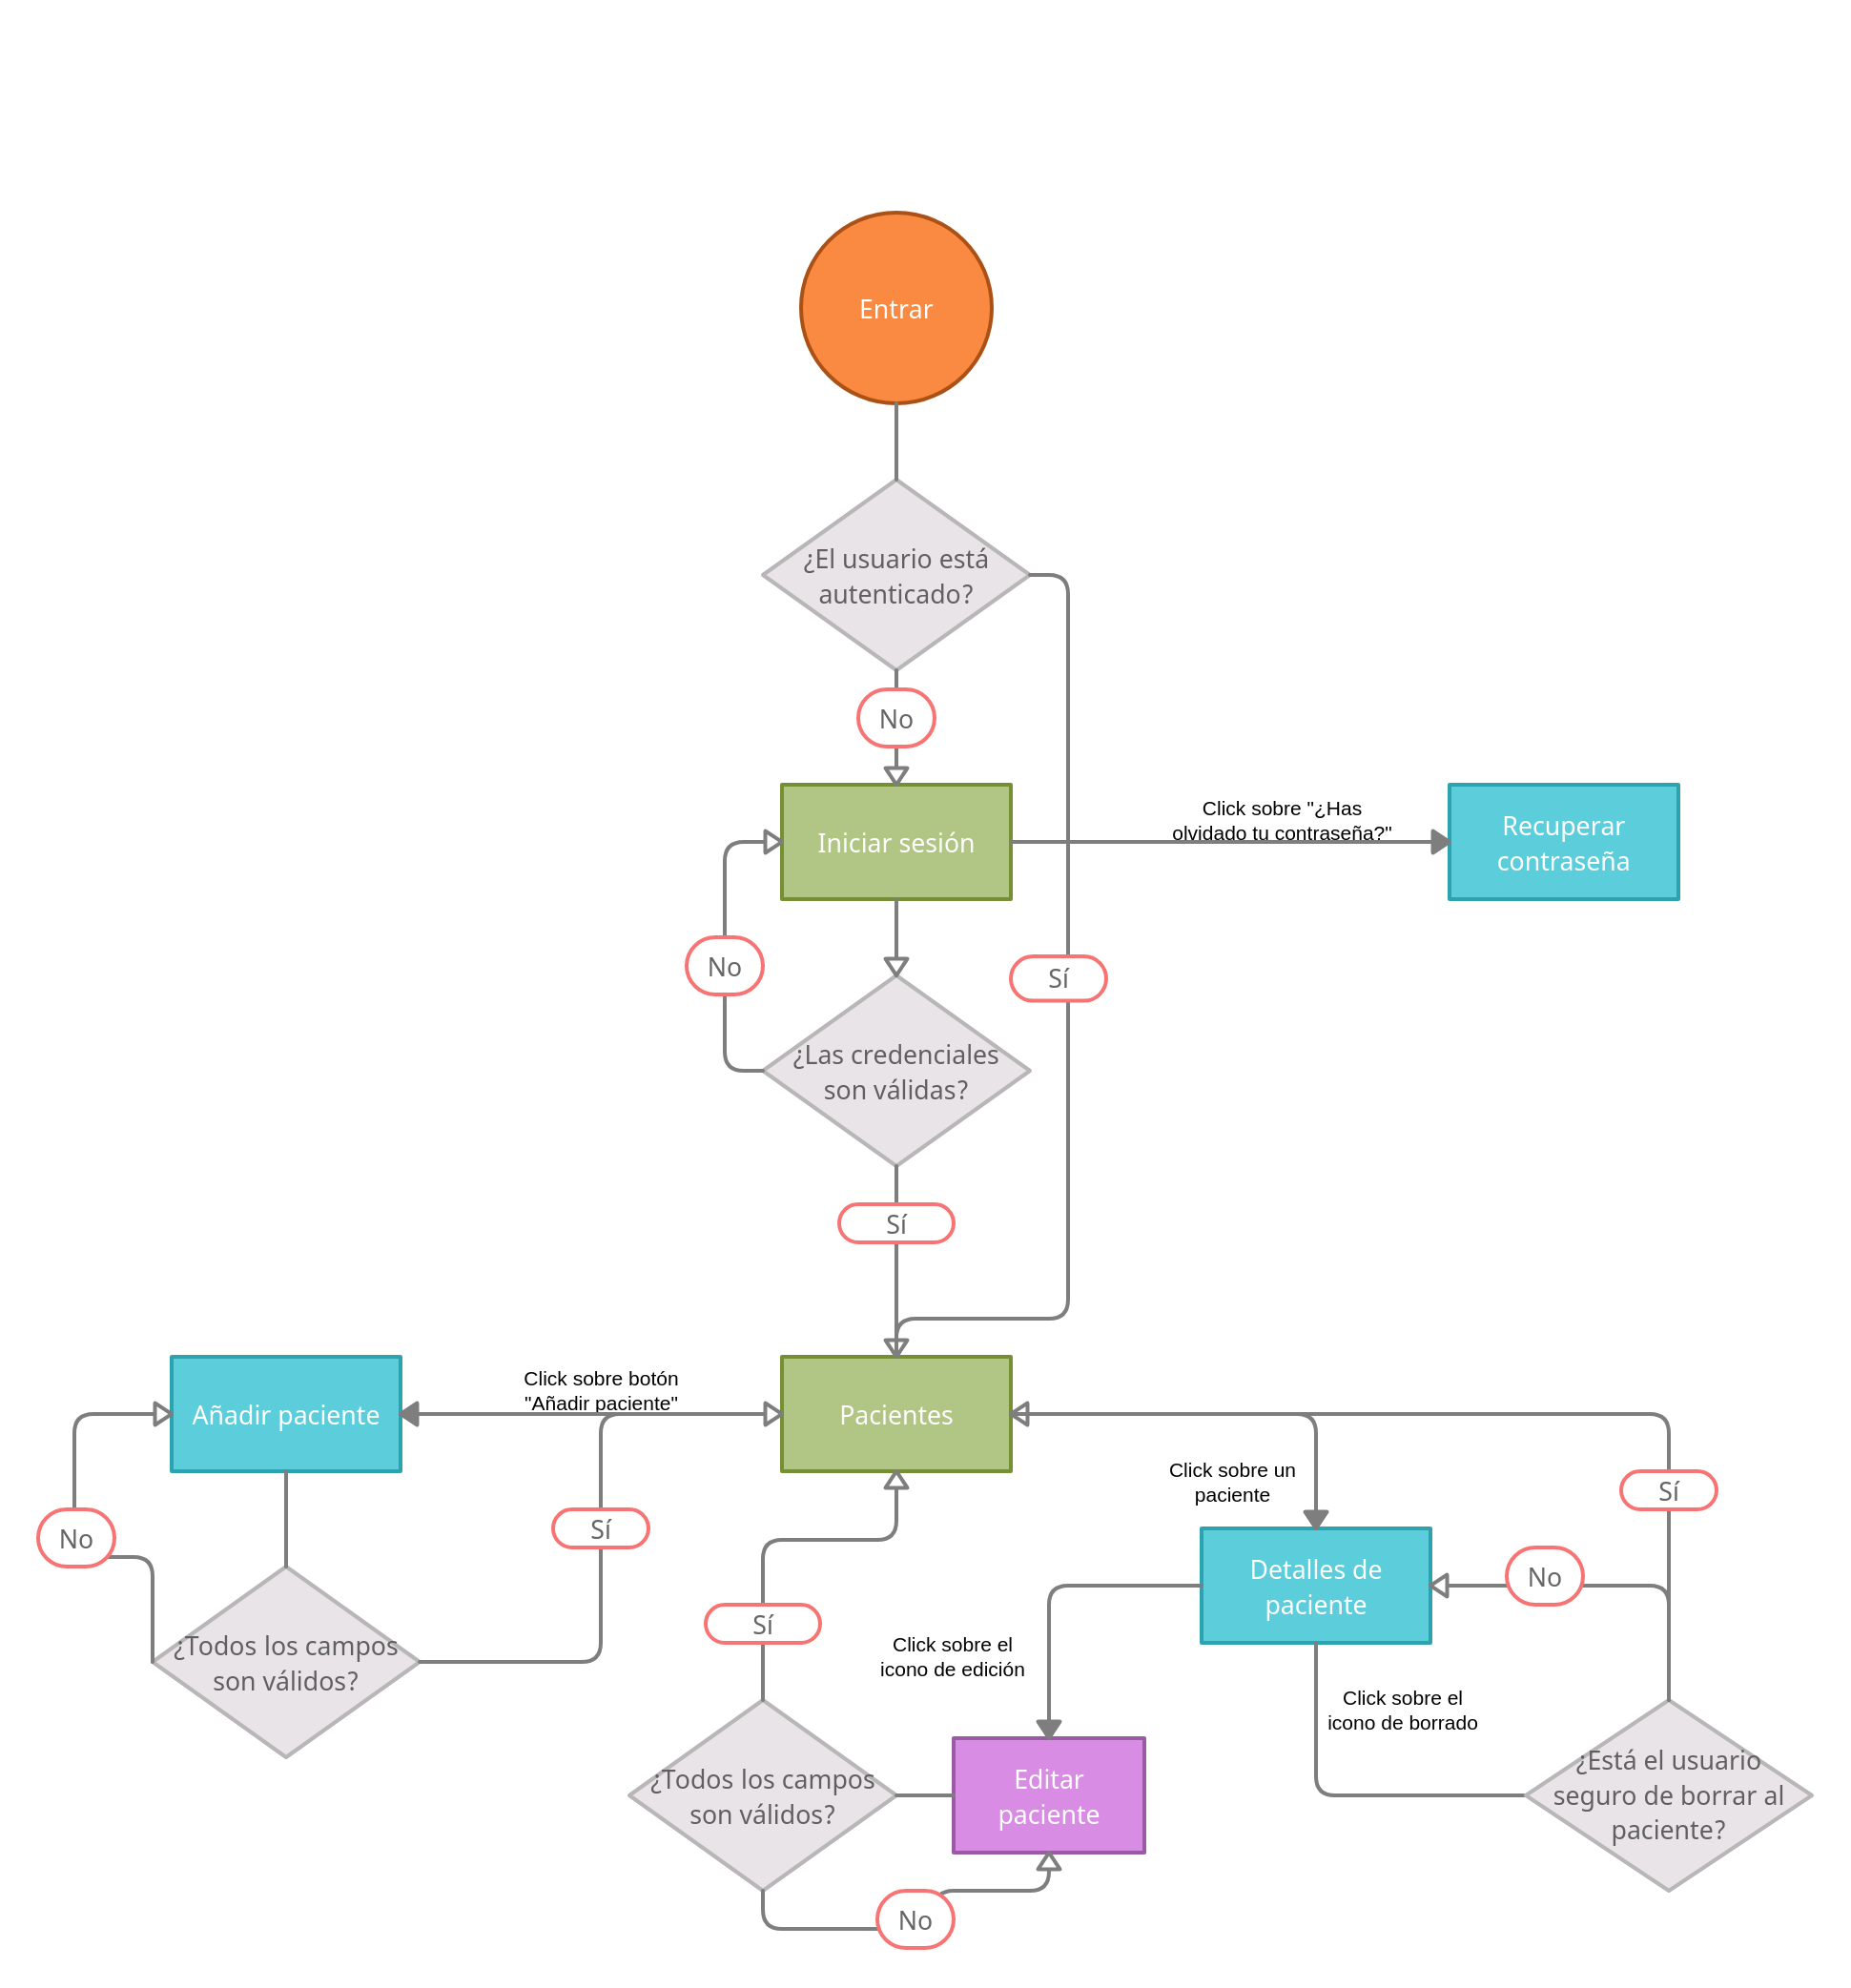
\includegraphics[scale=0.1]{doc/imagenes/flow-pacientes.png}}
    \caption{Flujo de usuario para la sección de Pacientes}
    \label{flow-pacientes}
\end{figure}

\begin{figure}[H]
    \centering{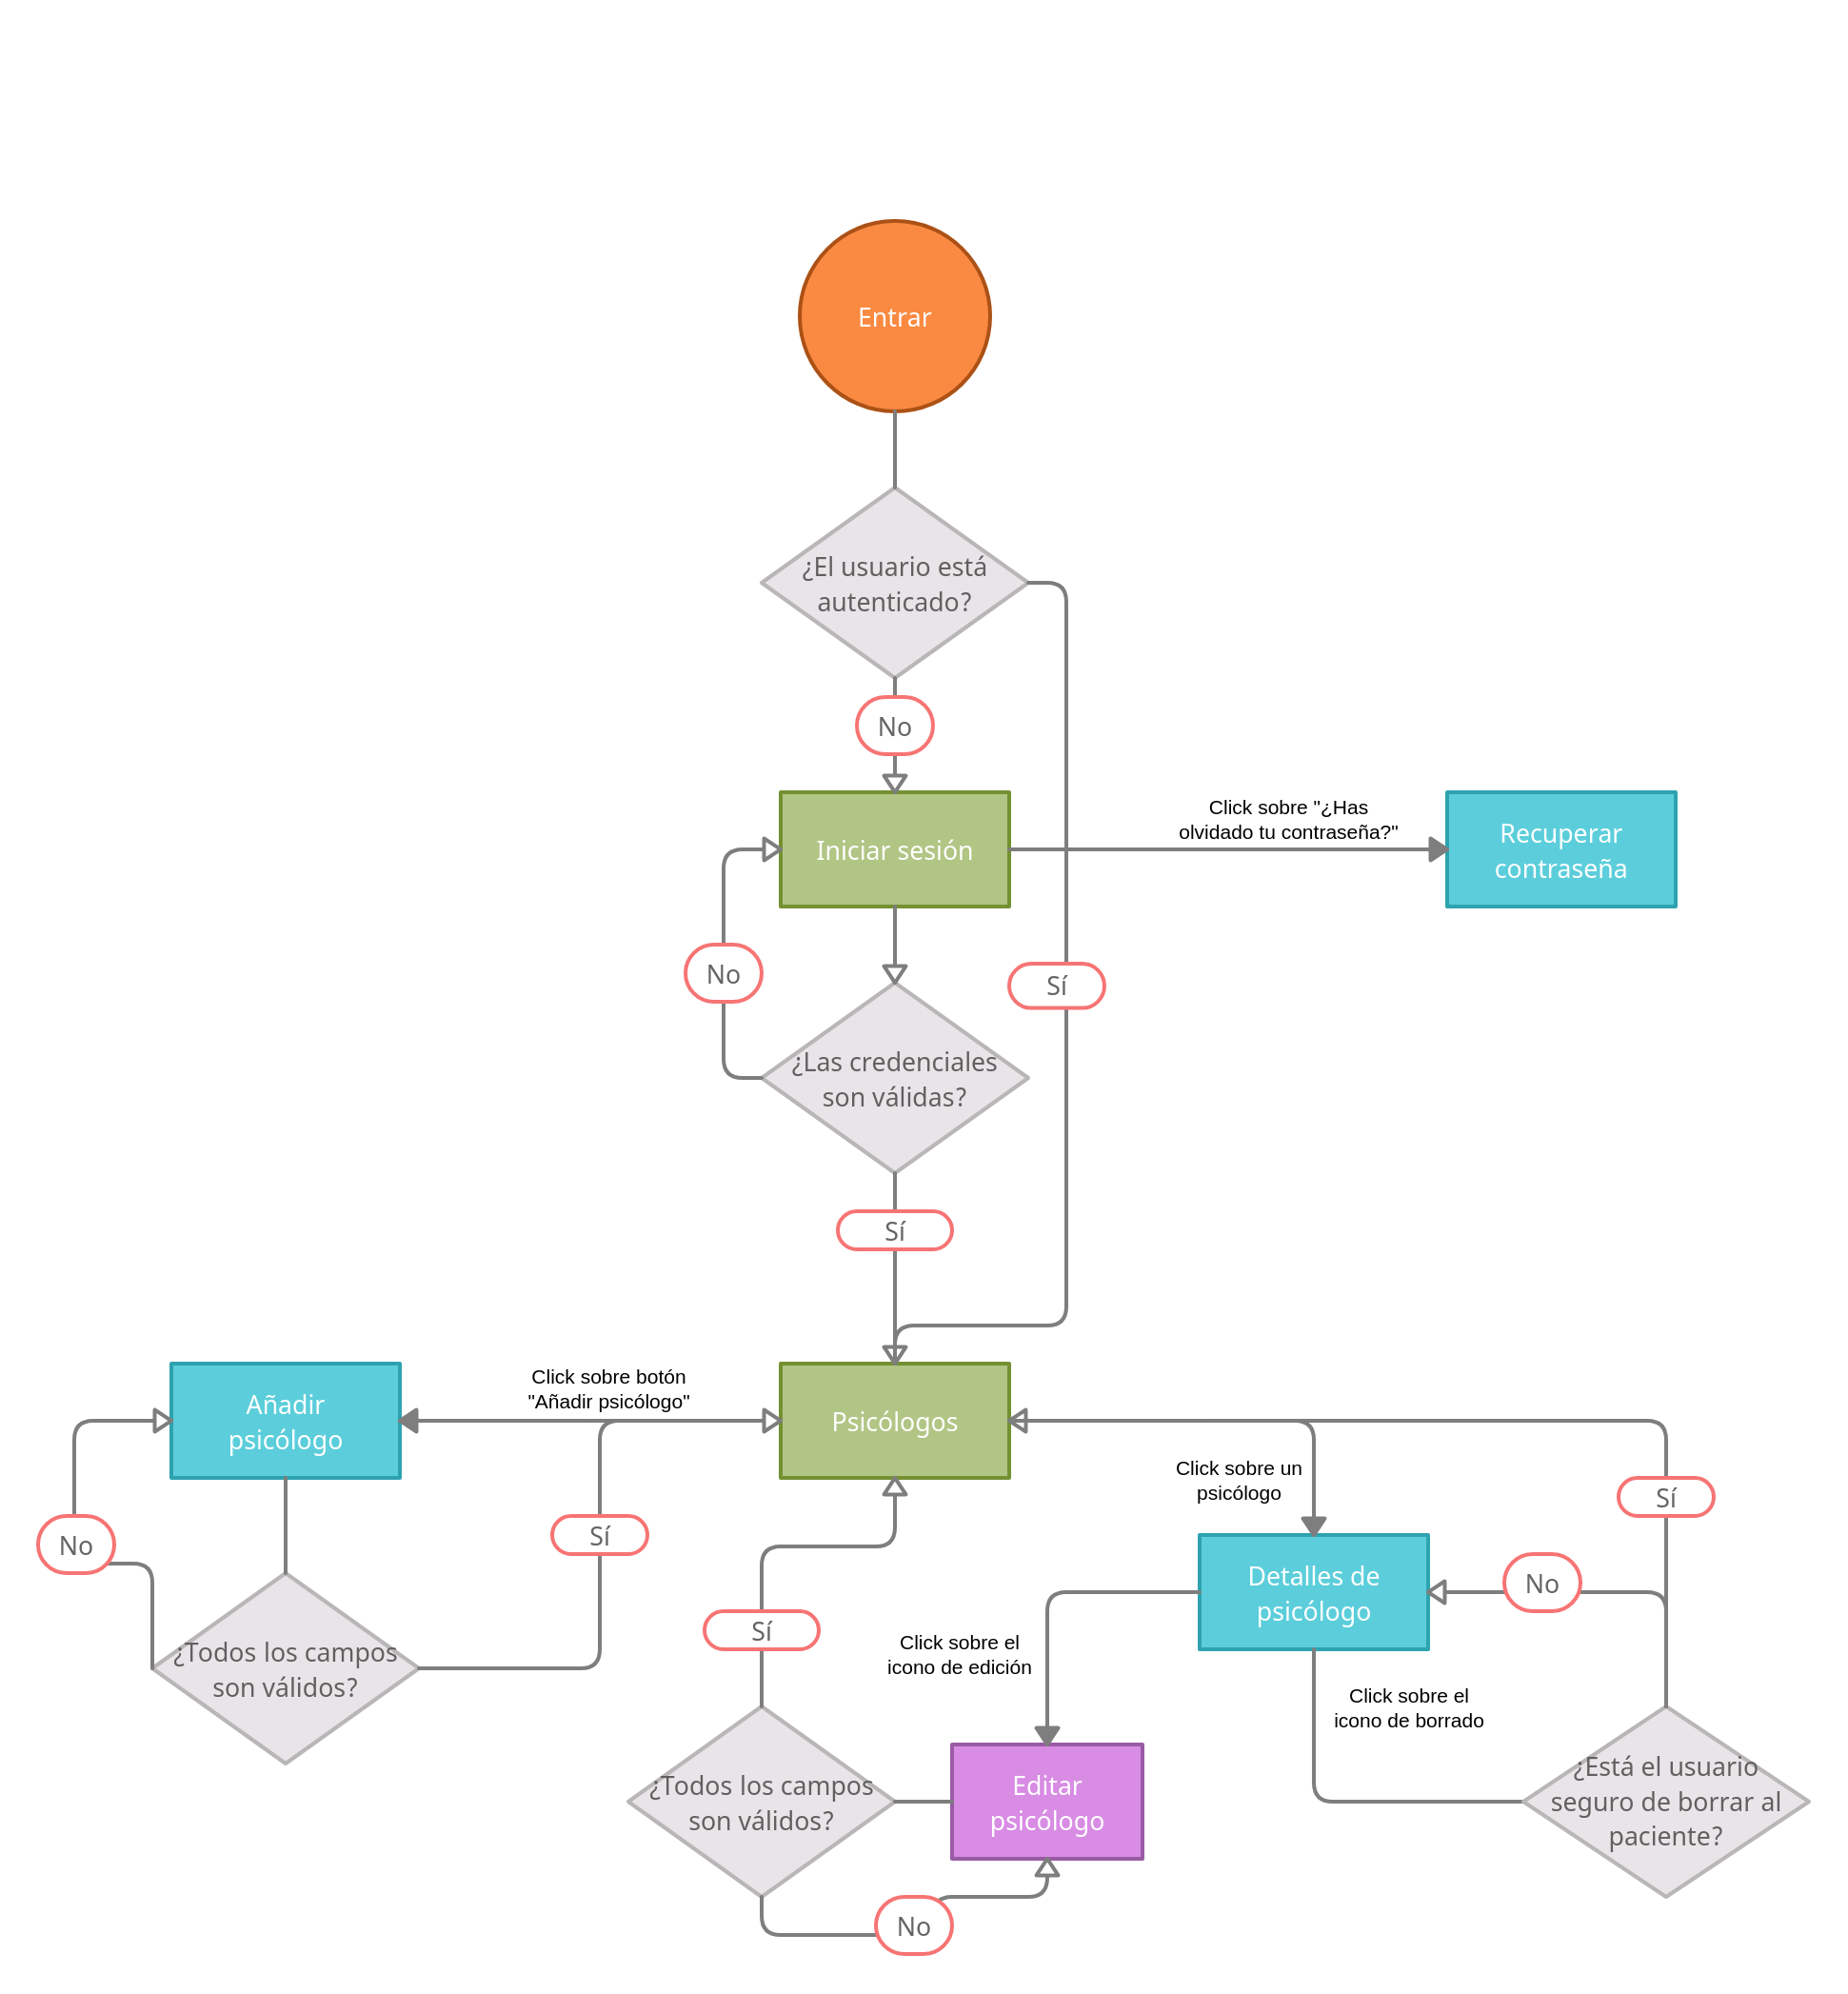
\includegraphics[scale=0.1]{doc/imagenes/flow-psicologos.png}}
    \caption{Flujo de usuario para la sección de Psicólogos}
    \label{flow-psicologos}
\end{figure}

Finalmente a estos flujos de usuario se añade el flujo de usuario de la sección de Perfil (Figura \ref{flow-perfil}).

\begin{figure}[H]
    \centering{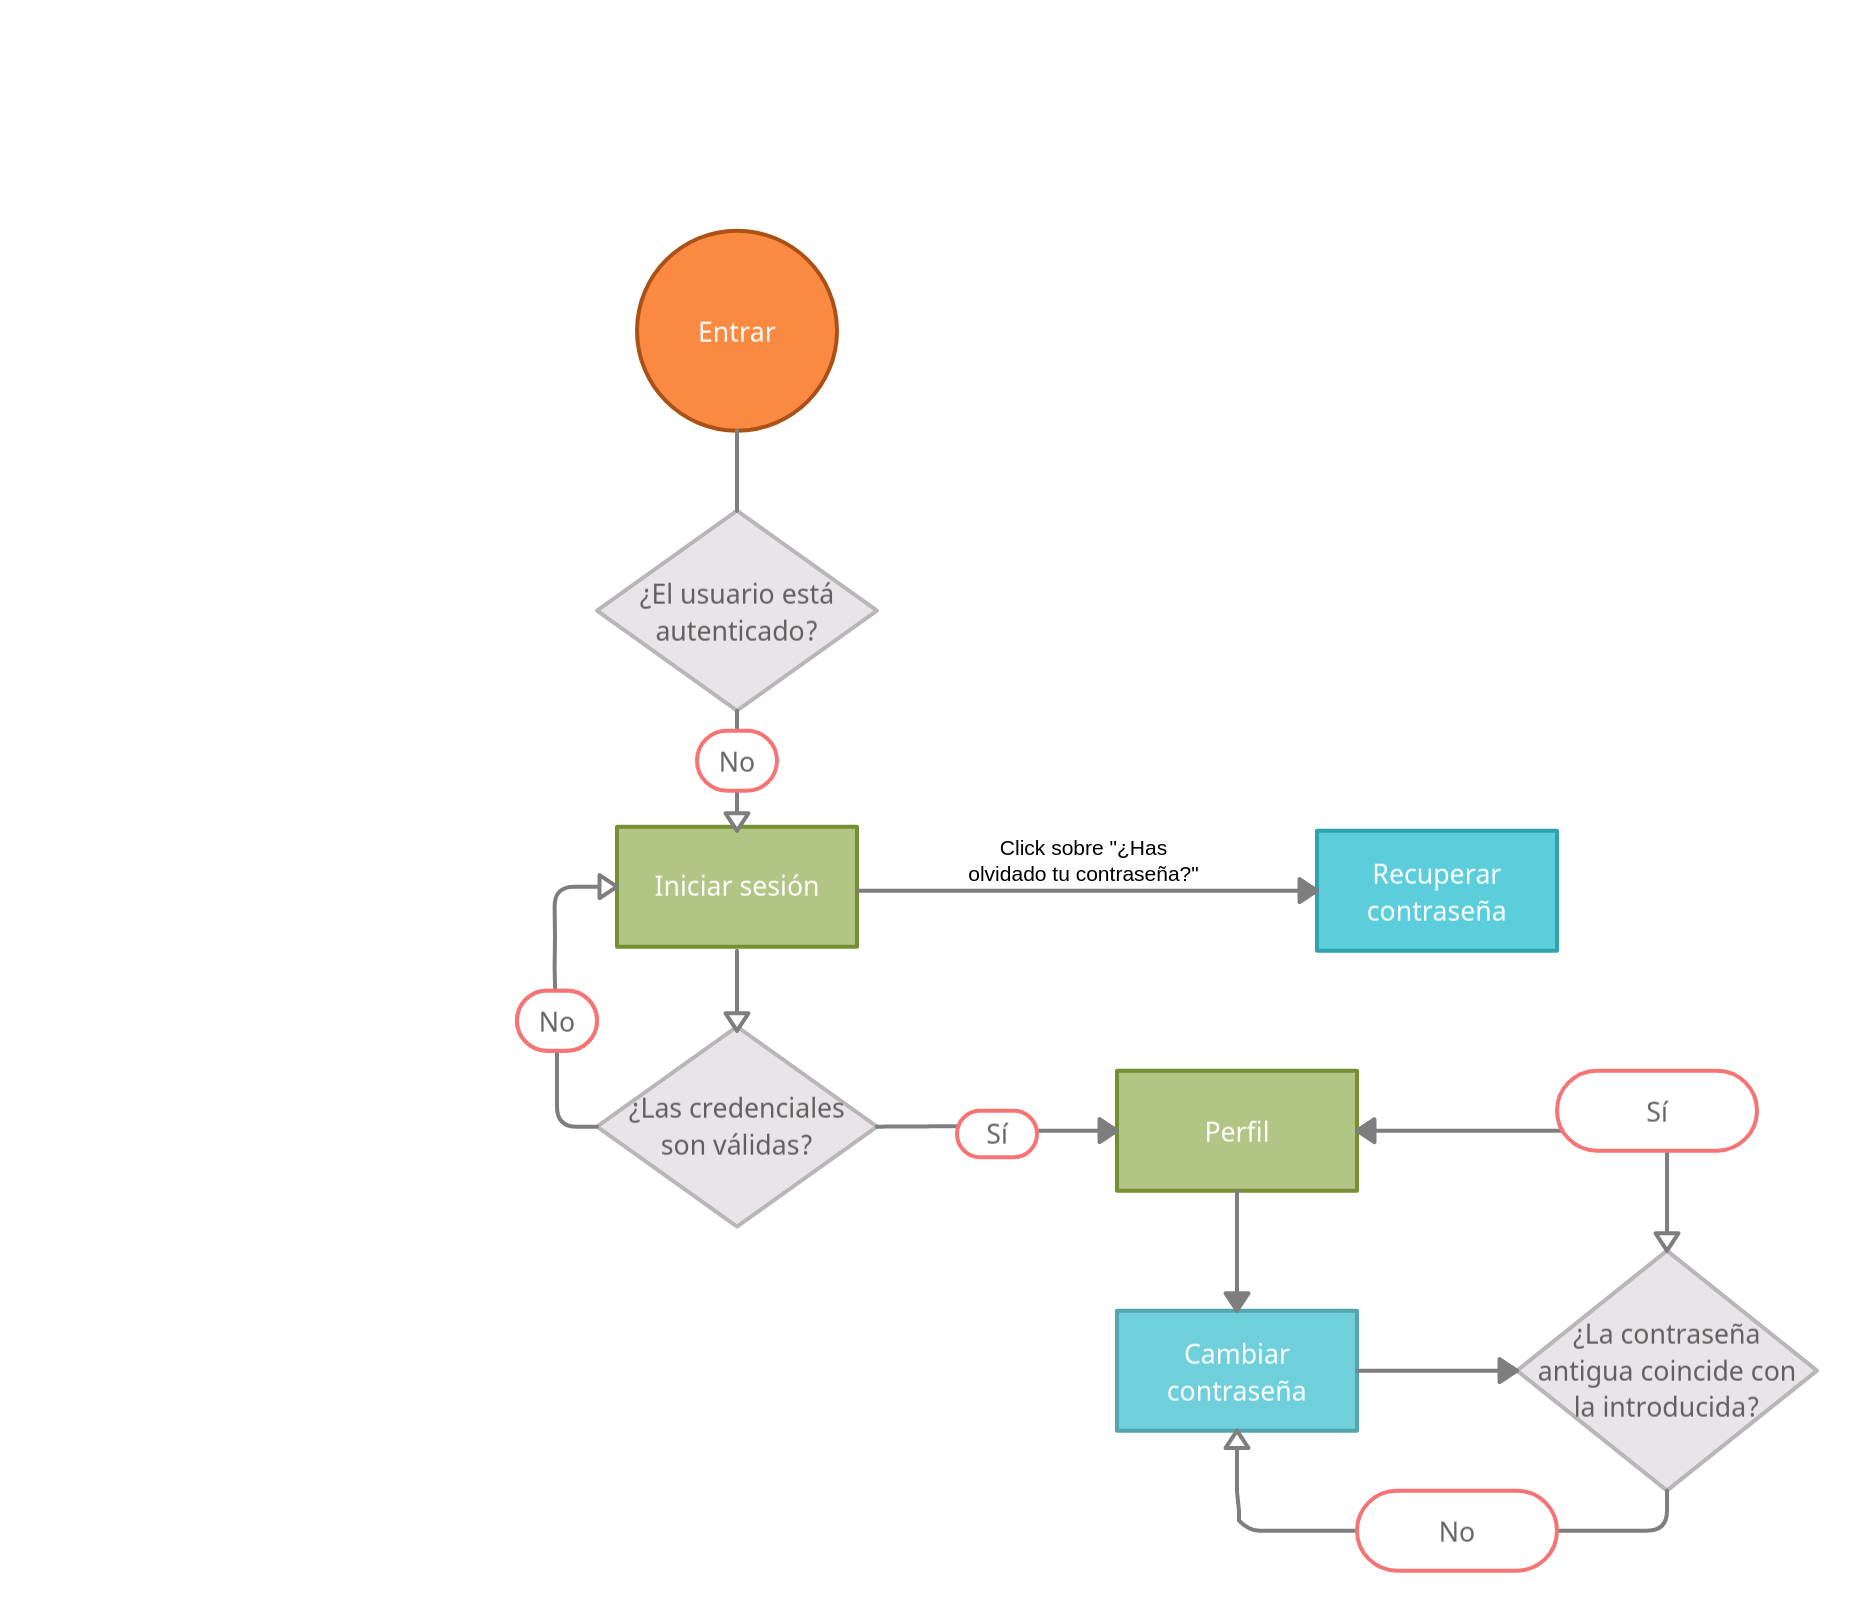
\includegraphics[scale=0.1]{doc/imagenes/flow-perfil.png}}
    \caption{Flujo de usuario para la sección de Perfil}
    \label{flow-perfil}
\end{figure}


Una vez ha sido definido el flujo de usuario en la plataforma, es momento de la parte más creativa del diseño en la que se definirá la actitud que se pretende transmitir a los usuarios y con ello se escogerá un nombre para la web, una paleta de colores, la elección de una fuente apropiada, un eslogan y la creación de un logo. \bigskip

Para establecer el tono y voz utilizado en la web se ha de tener en cuenta el contexto en el que se encuentra, el cual es el de un centro sanitario. Por tanto, el contenido que se va a ofrecer a los usuarios debe de ser profesional y serio. En consecuencia, la plataforma será lo más directa posible mostrando de forma clara las acciones a realizar en ella, así como los errores que se puedan dar. A su vez, se buscará transmitir una actitud calmada evitando el uso de palabras en mayúsculas o signos de exclamación. Ahora bien, a pesar de este tono profesional naturalmente no se ha de olvidar la cercanía que en todo momento se procura tener con los pacientes en el ámbito de la salud.\bigskip

Teniendo claro lo anterior, es hora de elegir un nombre para la plataforma. Para su elección se han tenido numerosas ideas combinando los conceptos de tiempo y cita médica como ''HTime'', ''Mediatrics'', ''HeyPlannect'',''iAppointment'', ''Dation'', etc. Sin embargo, finalmente la opción elegida ha sido \textbf{''DayDay''} por su sencillez y facilidad para recordar. De igual forma para el eslogan se barajaron múltiples opciones, pero finalmente se escogió ''365 días en una página'' por las mismas razones. \bigskip

En cuanto a la elección de la paleta de colores, teniendo presente la actitud a transmitir a los usuarios que se ha definido anteriormente, se va a seguir para su elección el artículo escrito por Jicheng Yang y Xiaoying Shen ''The Application of Color Psychology in Community Health
Environment Design'' \cite{Yang2022} en el que se exponen los resultados obtenidos a través de una investigación llevada a cabo sobre la psicología del color en el ámbito de la salud. Yang y Shen afirman que cada color tiene su propia personalidad. Seguidamente se muestra en la Figura \ref{psicologia-color} los rasgos que representan a cada color:

\begin{figure}[H]
    \centering{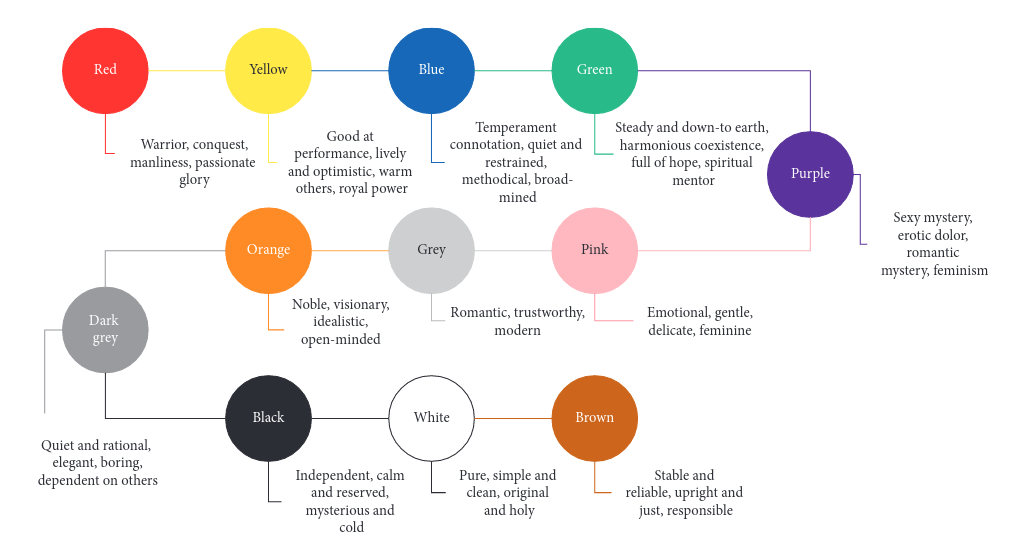
\includegraphics[scale=0.4]{doc/imagenes/psicologia-color.png}}
    \caption{Rasgos de personalidad del color \cite{Yang2022}}
    \label{psicologia-color}
\end{figure}

A través de dicha figura se observan ciertos rasgos con los que DayDay se identifica: la sencillez y pureza del blanco, la harmonía del verde, la paz del azul, la fiabilidad del marrón, la confianza del gris o la nobleza del naranja. Tomando en consideración esto y buscando un diseño lo más accesible posible, se ha elegido la siguiente paleta (Figura \ref{paleta}) por sus contrastres:

\begin{figure}[H]
    \centering{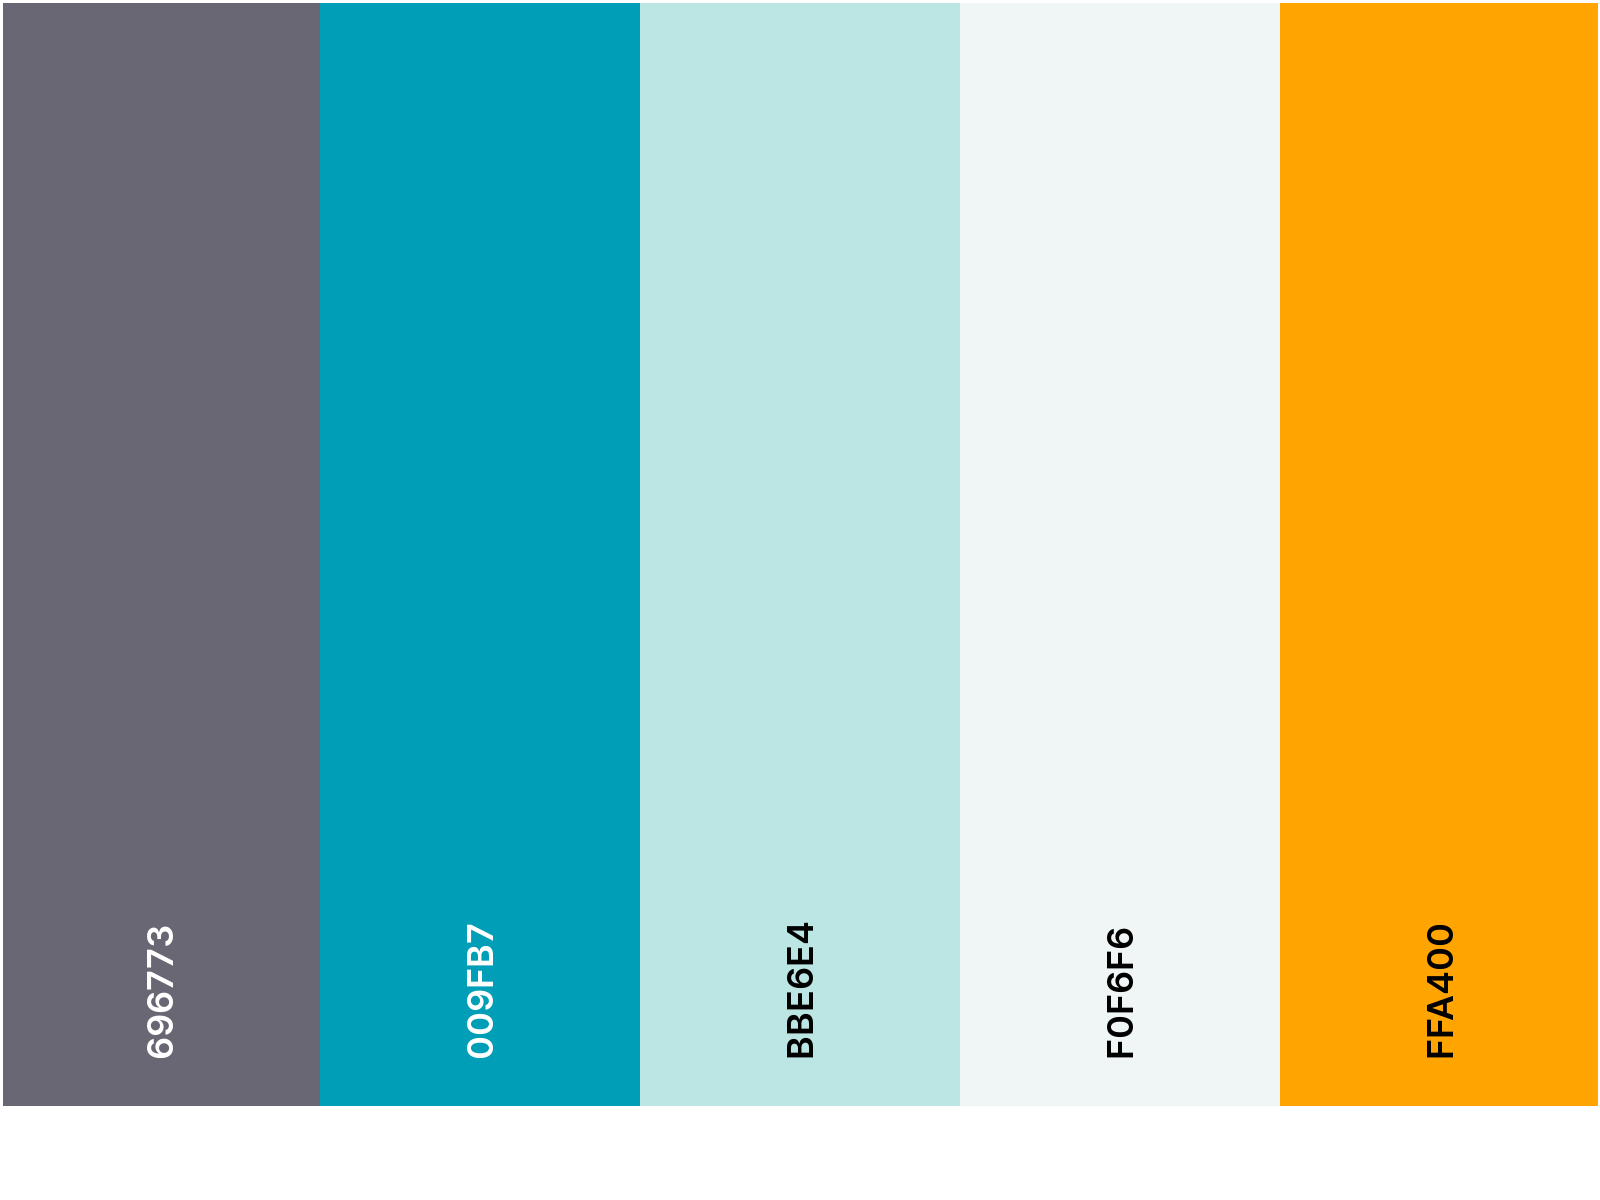
\includegraphics[scale=0.15]{doc/imagenes/DayDay_palette.png}}
    \caption{Paleta de colores de DayDay}
    \label{paleta}
\end{figure}

Como se ha comentado, también se ha de elegir una fuente para la plataforma y ésta debe de ser accesible para usuarios con dislexia o con alguna discapacidad visual. La fuente utilizada por Google Material es ''Roboto'' (Figura \ref{roboto}), la cual es una fuente ''sans-serif'', lo cual significa que Roboto utiliza caracteres simples que se diferencian claramente los unos de los otros por lo que falicita la lectura a los tipos de usuarios mencionados.

\begin{figure}[H]
    \centering{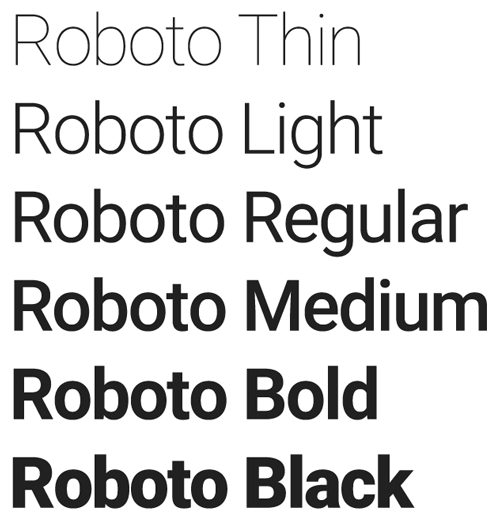
\includegraphics[scale=0.2]{doc/imagenes/roboto.png}}
    \caption{Fuente ''Roboto'' de Google Material}
    \label{roboto}
\end{figure}

Además, se seguirán los siguientes tamaños de fuente proporcionados por la guía de diseño de Google Material para los distintos formatos de texto (Figura \ref{font-size}):

\begin{figure}[H]
    \centering{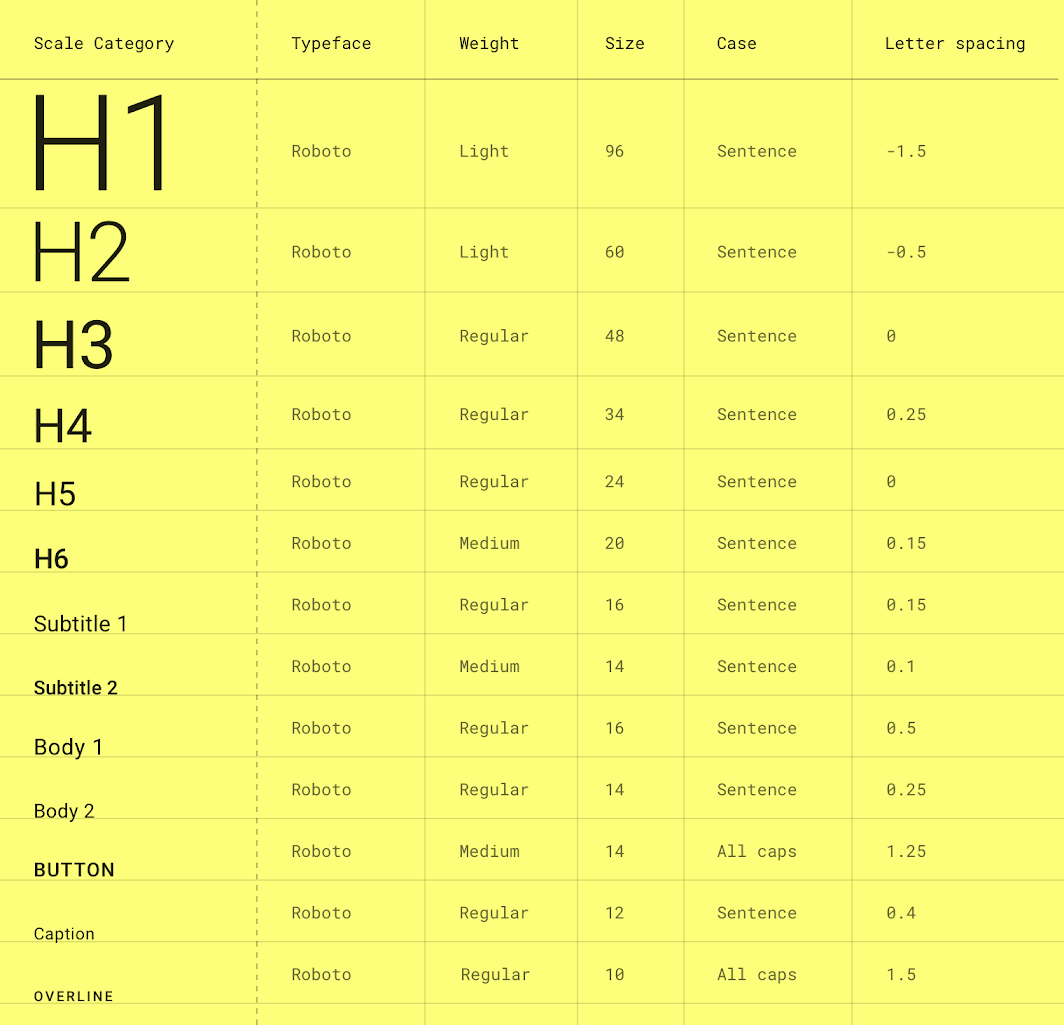
\includegraphics[scale=0.2]{doc/imagenes/font-size.png}}
    \caption{Tamaños de fuente para ''Roboto'' según las guías de diseño de Google Material}
    \label{font-size}
\end{figure}

Finalmente, a continuación se muestra el logo de DayDay (Figura \ref{logo-dayday}), el cual ha sido diseñado en el editor online Figma:

\begin{figure}[H]
    \centering{
\includegraphics[scale=0.1]{doc/imagenes/DayDay_logo.png}}
    \caption{Logo de DayDay}
    \label{logo-dayday}
\end{figure}

Como cuadro resumen de lo explicado, se recoge todo lo expuesto anteriormente en el siguiente Moodboard (Figura \ref{moodboard}):

\begin{figure}[H]
    \centering{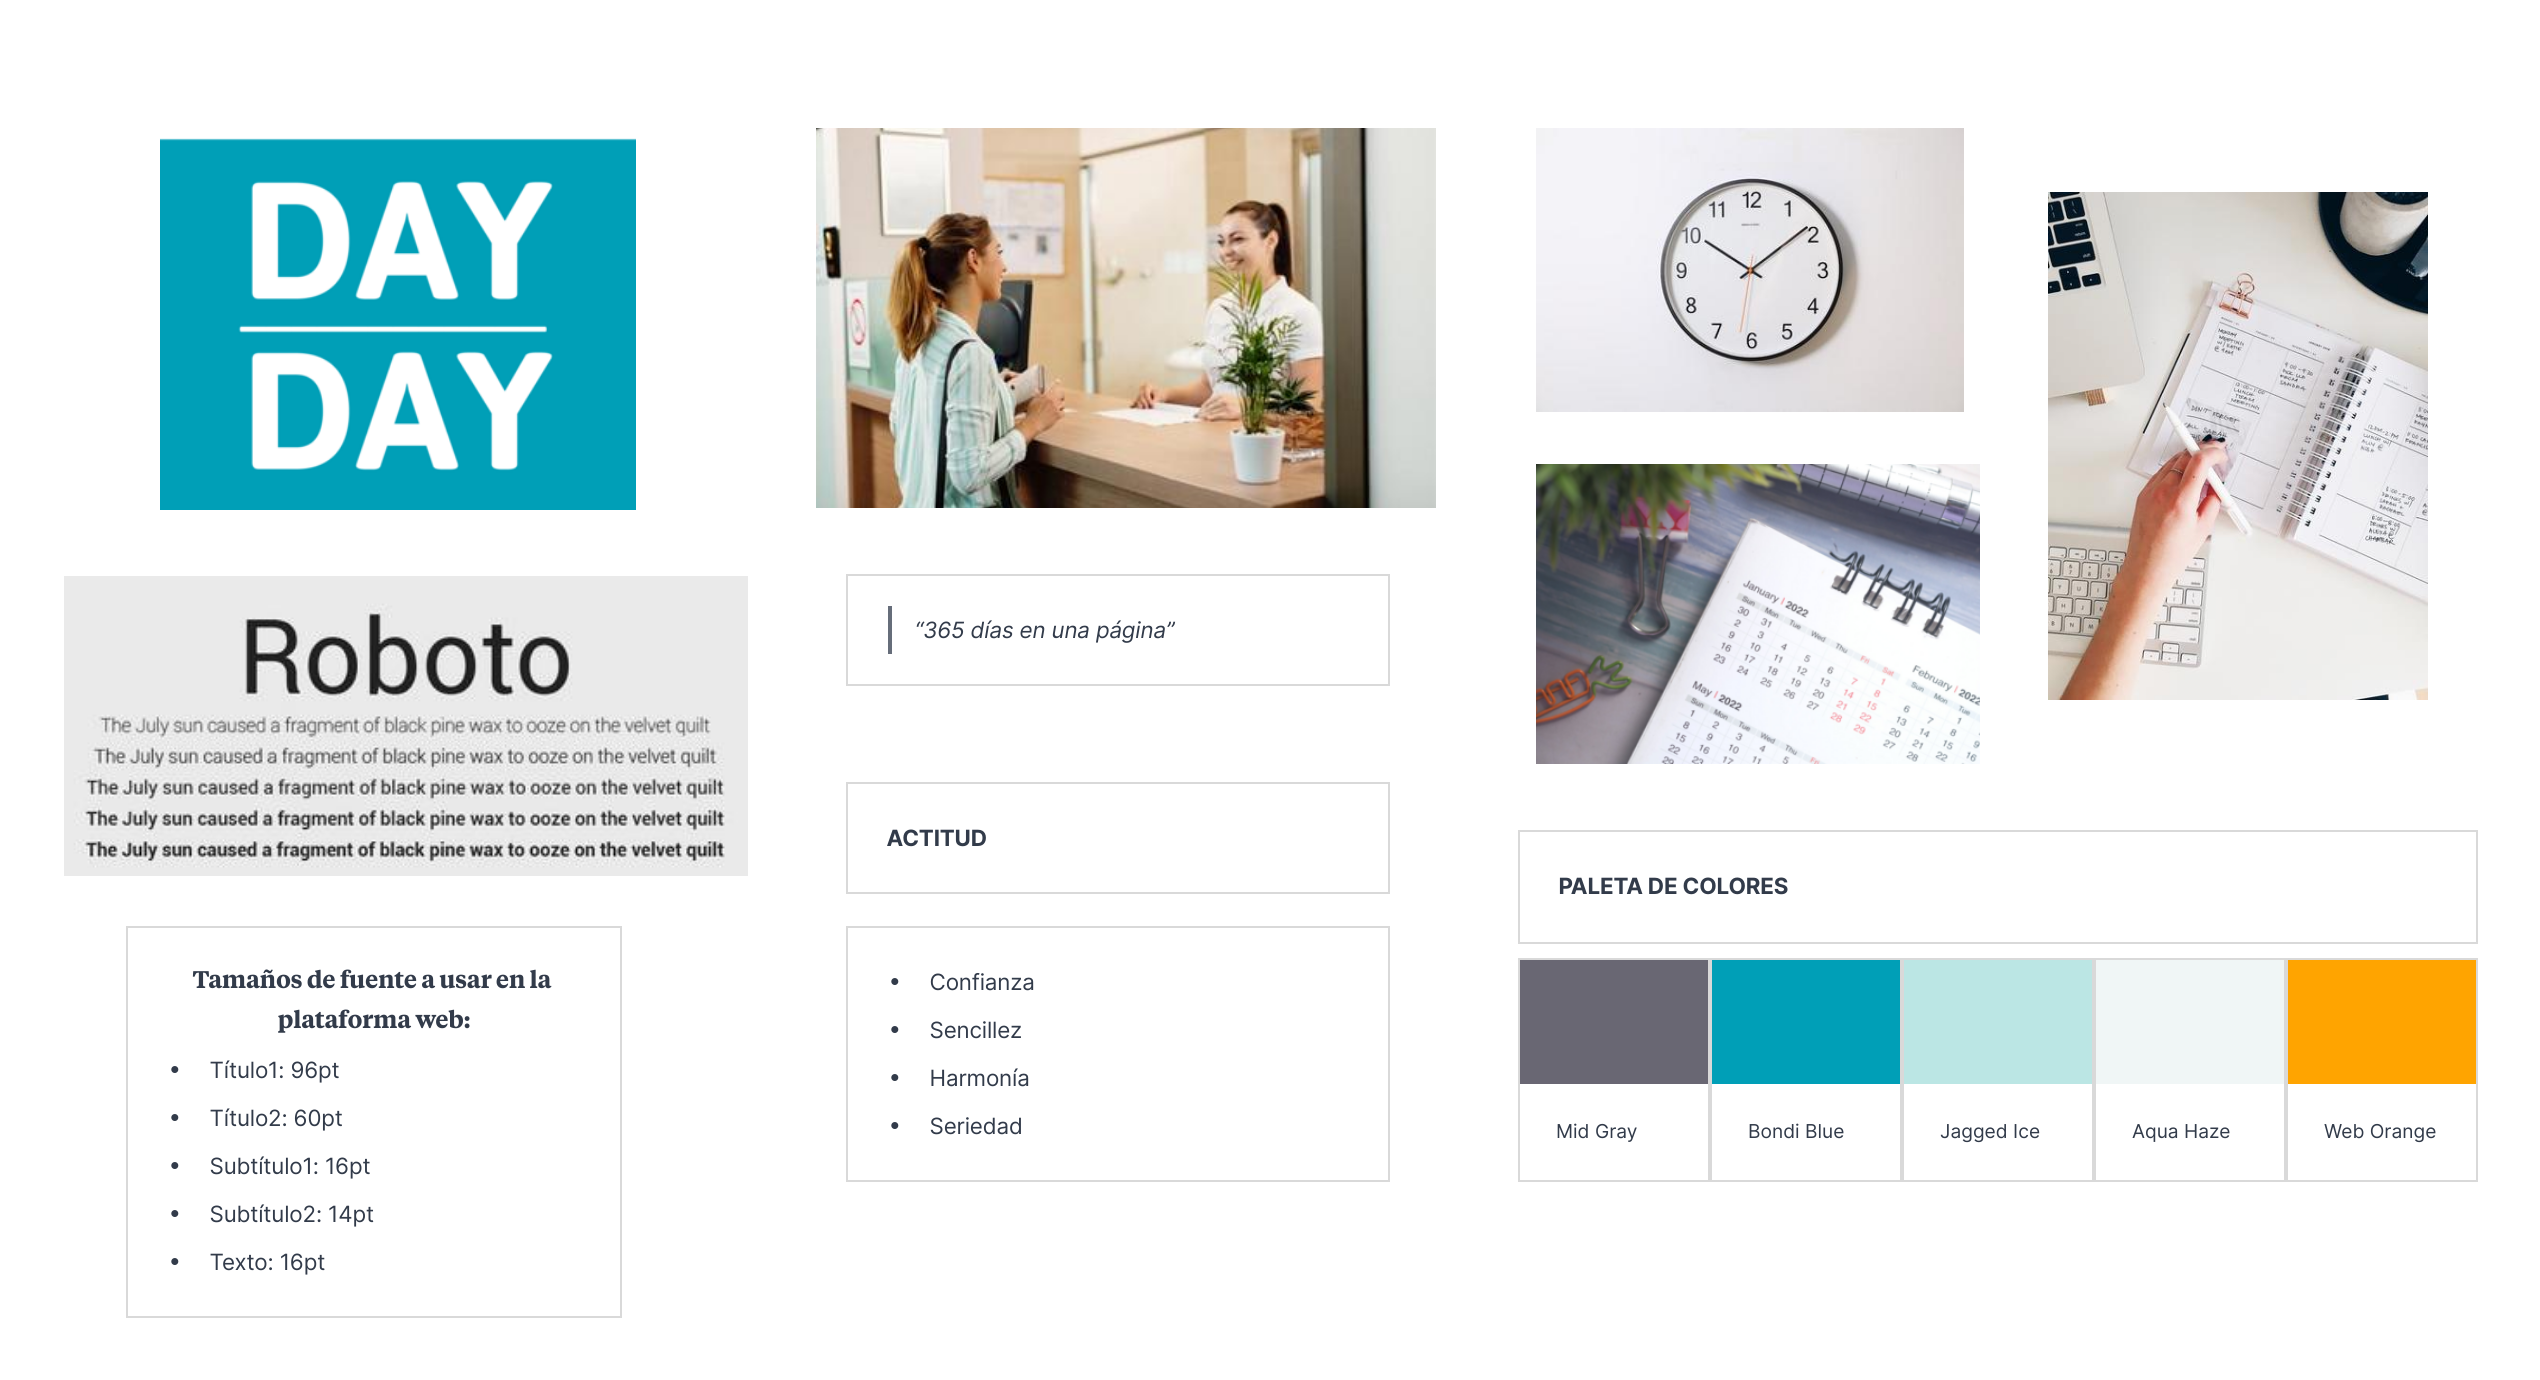
\includegraphics[scale=0.15]{doc/imagenes/moodboard.png}}
    \caption{Moodboard de DayDay}
    \label{moodboard}
\end{figure}

\subsubsection{Wireframes y Mockups} \label{mockup-wirefram}
Tras implantar las guías de diseño que seguirá DayDay es momento de crear los diseños de la interfaz, para ello utilizamos la herramienta Figma.

Primeramente se han preparado unos wireframes que servirán para establecer el entramado de la interfaz de DayDay (Figuras \ref{wireframe-login}, \ref{wireframe-calendario}, \ref{wireframe-pacientes}, \ref{wireframe-psicologos}, \ref{wireframe-perfil}, \ref{wireframe-crear-cita}, \ref{wireframe-editar-cita} y \ref{wireframe-cambiar-contraseña} ):

\begin{figure}[H]
    \centering{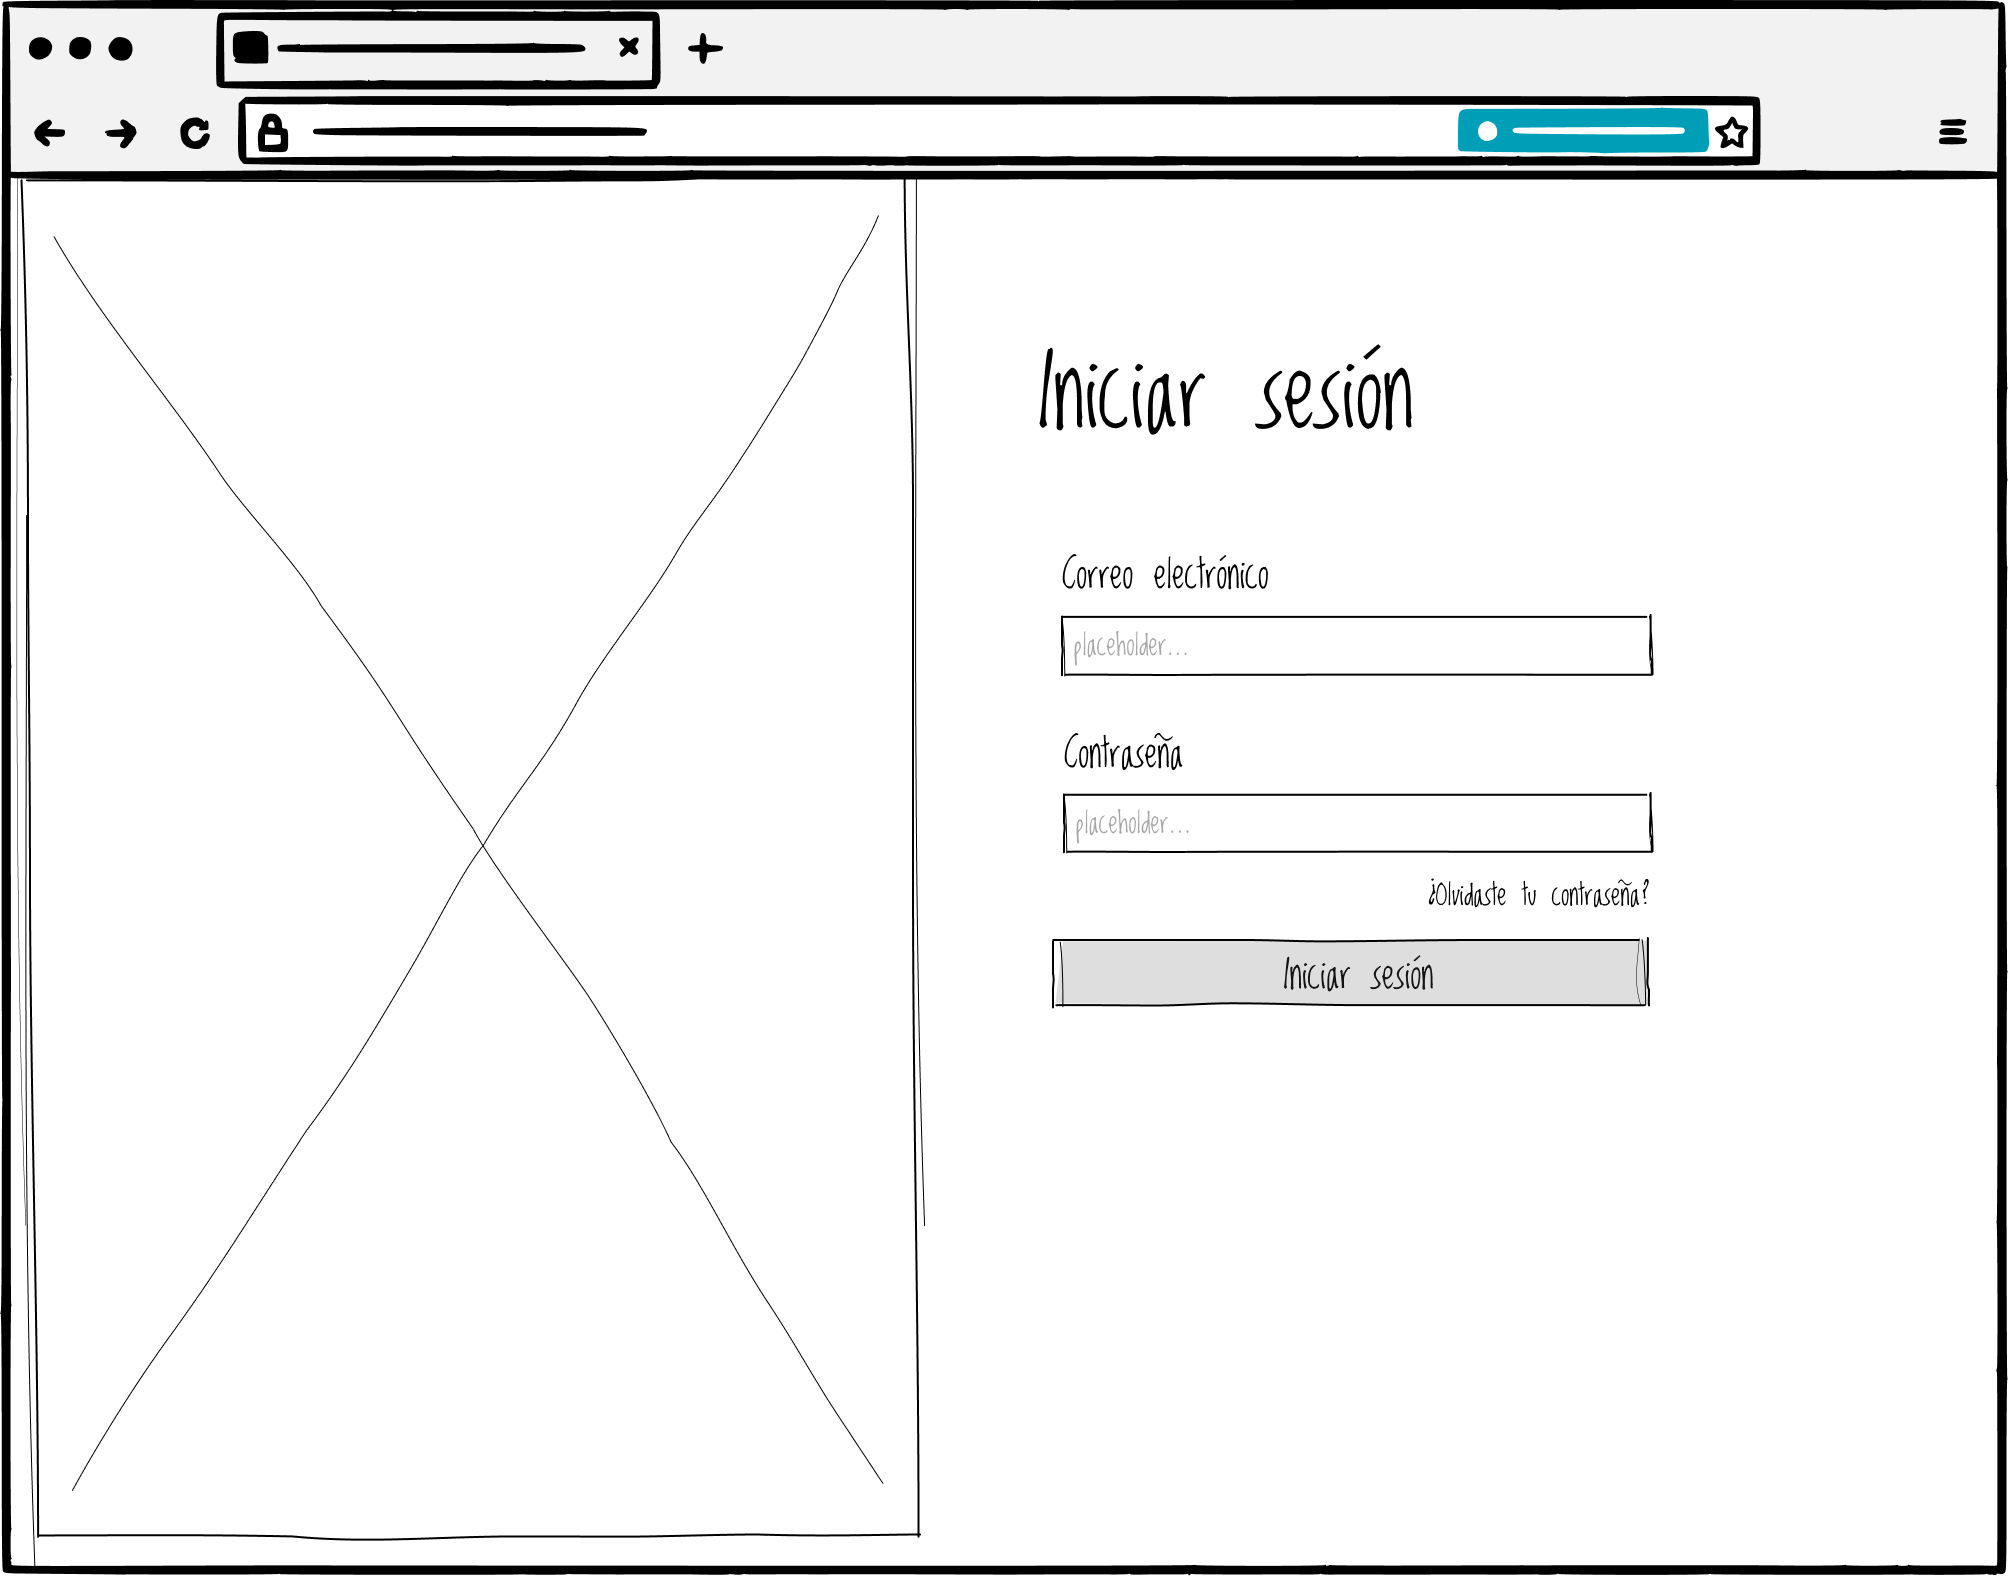
\includegraphics[scale=0.1]{doc/imagenes/vista-login.png}}
    \caption{Wireframe de la vista de Iniciar sesión}
    \label{wireframe-login}
\end{figure}

\begin{figure}[H]
    \centering{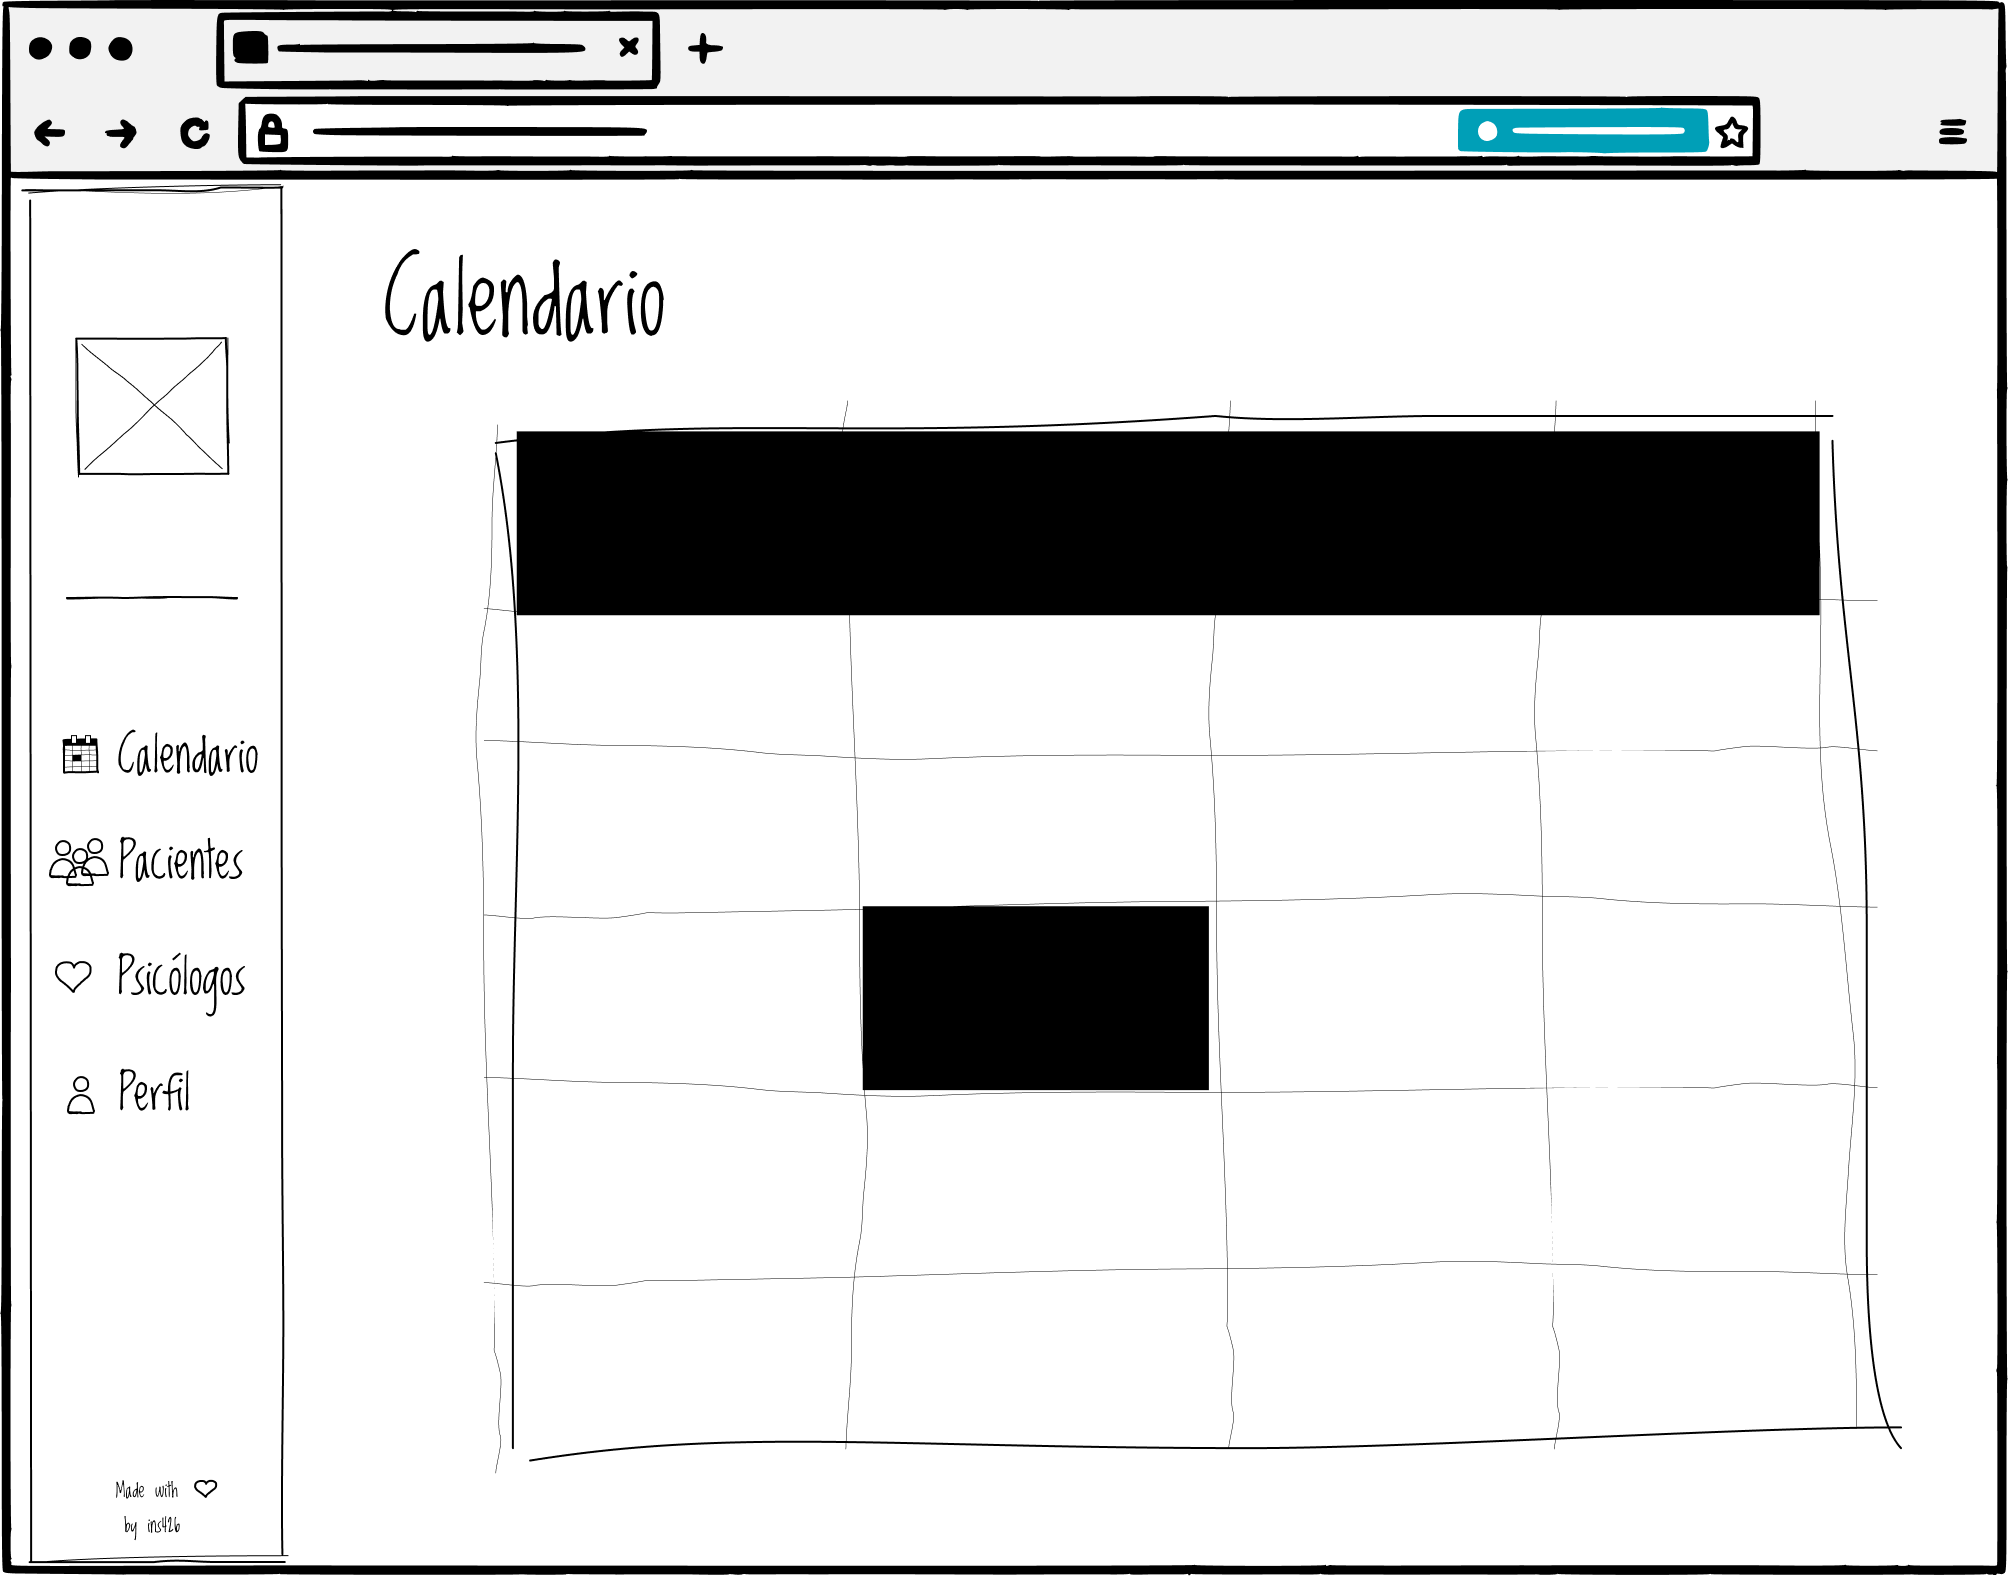
\includegraphics[scale=0.1]{doc/imagenes/vista-calendario.png}}
    \caption{Wireframe de la vista de Calendario}
    \label{wireframe-calendario}
\end{figure}

\begin{figure}[H]
    \centering{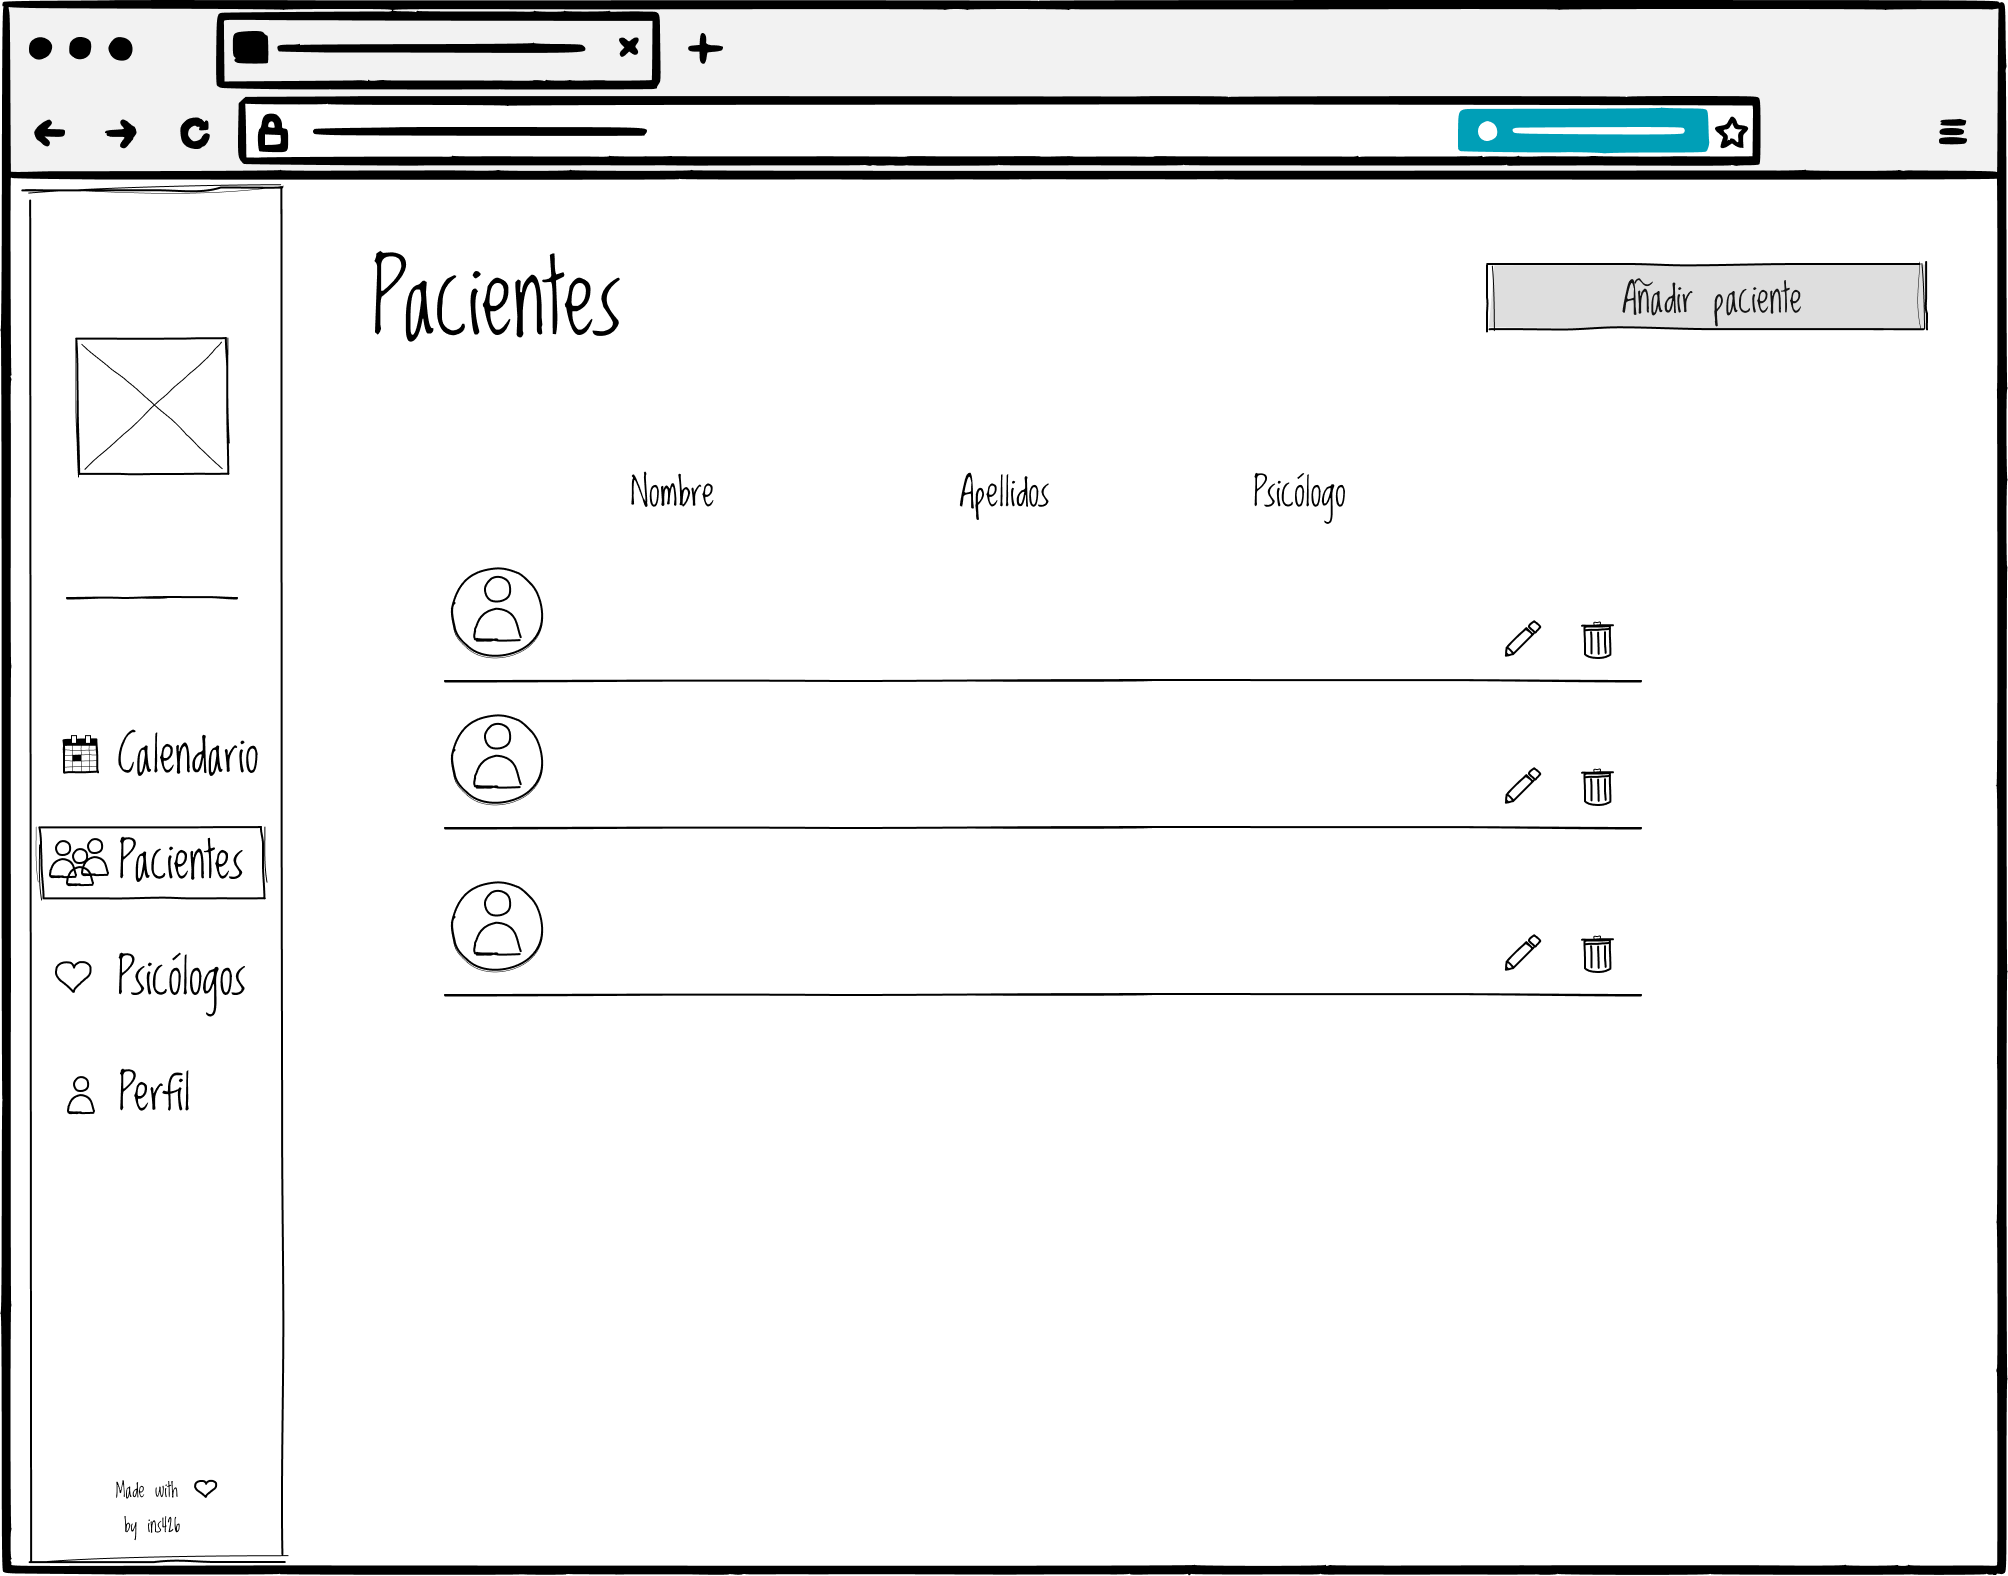
\includegraphics[scale=0.1]{doc/imagenes/vista-pacientes.png}}
    \caption{Wireframe de la vista de Pacientes}
    \label{wireframe-pacientes}
\end{figure}

\begin{figure}[H]
    \centering{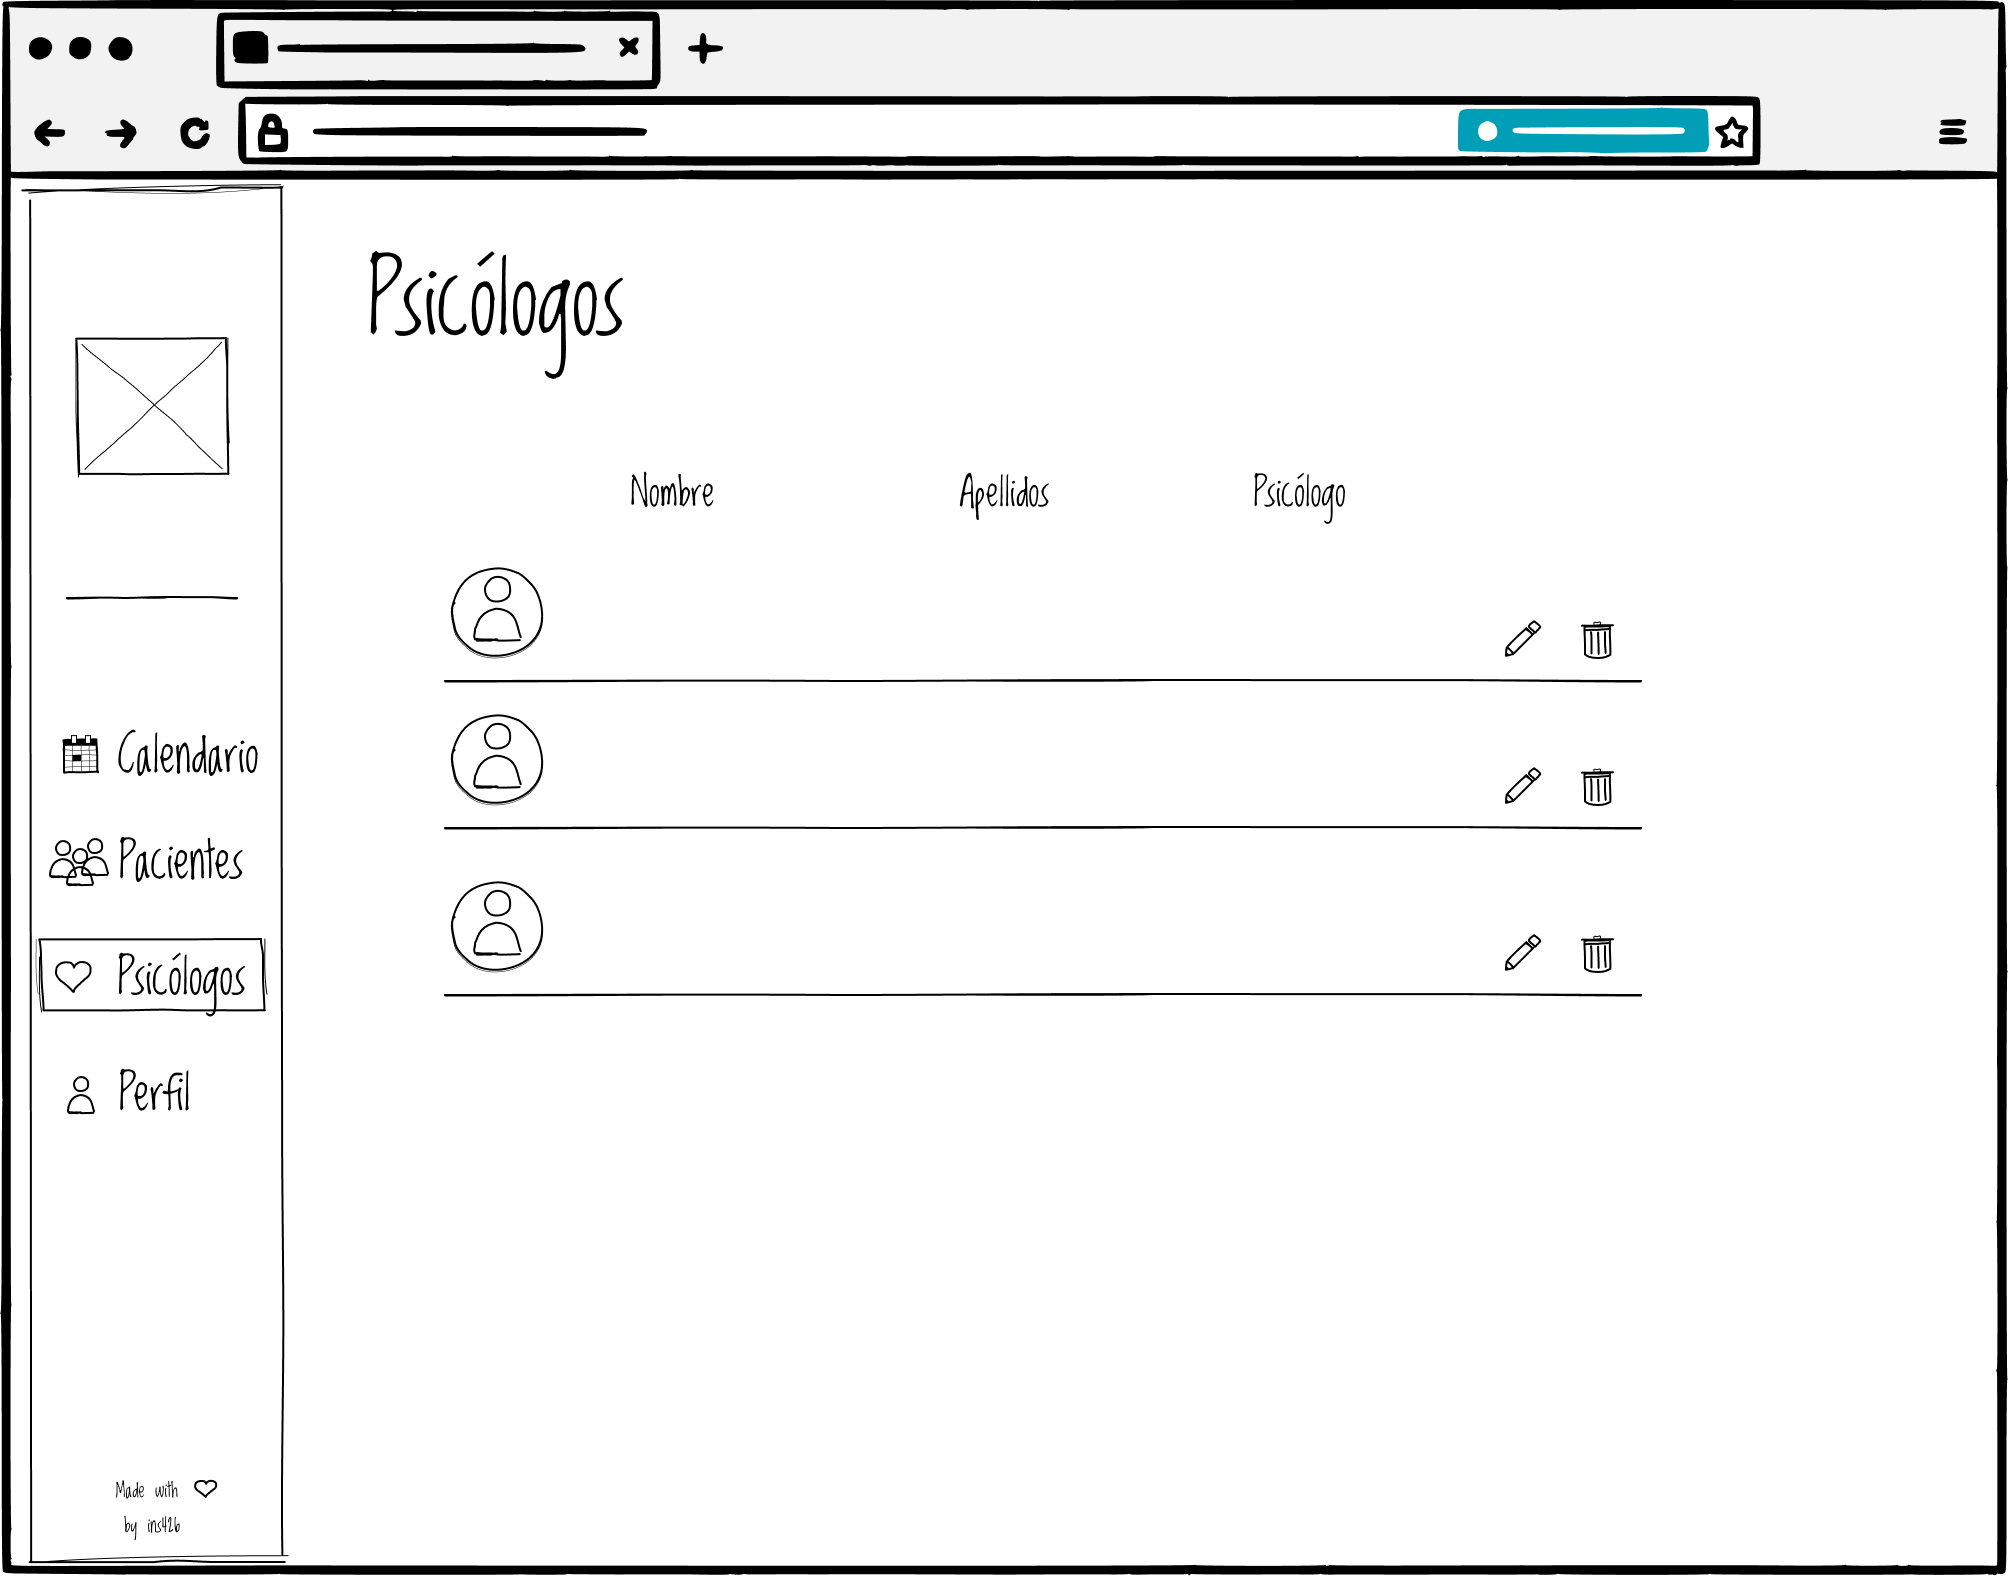
\includegraphics[scale=0.1]{doc/imagenes/vista-psicologos.png}}
    \caption{Wireframe de la vista de Psicólogos}
    \label{wireframe-psicologos}
\end{figure}

\begin{figure}[H]
    \centering{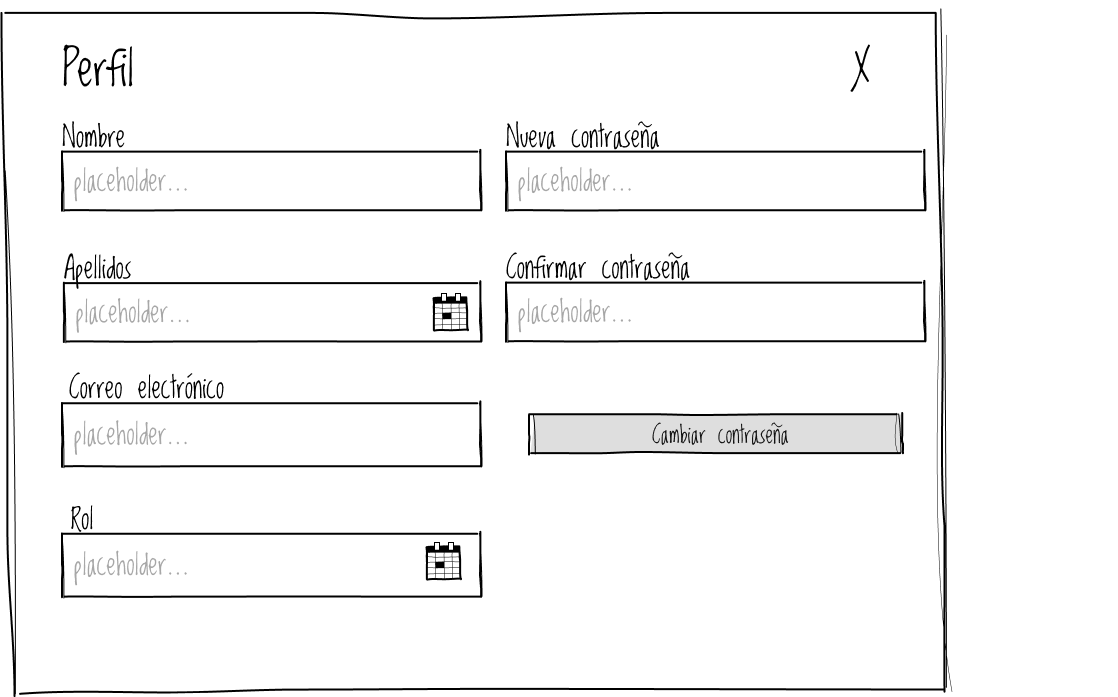
\includegraphics[scale=0.1]{doc/imagenes/vista-perfil.png}}
    \caption{Wireframe del diálogo de Perfil}
    \label{wireframe-perfil}
\end{figure}

\begin{figure}[H]
    \centering{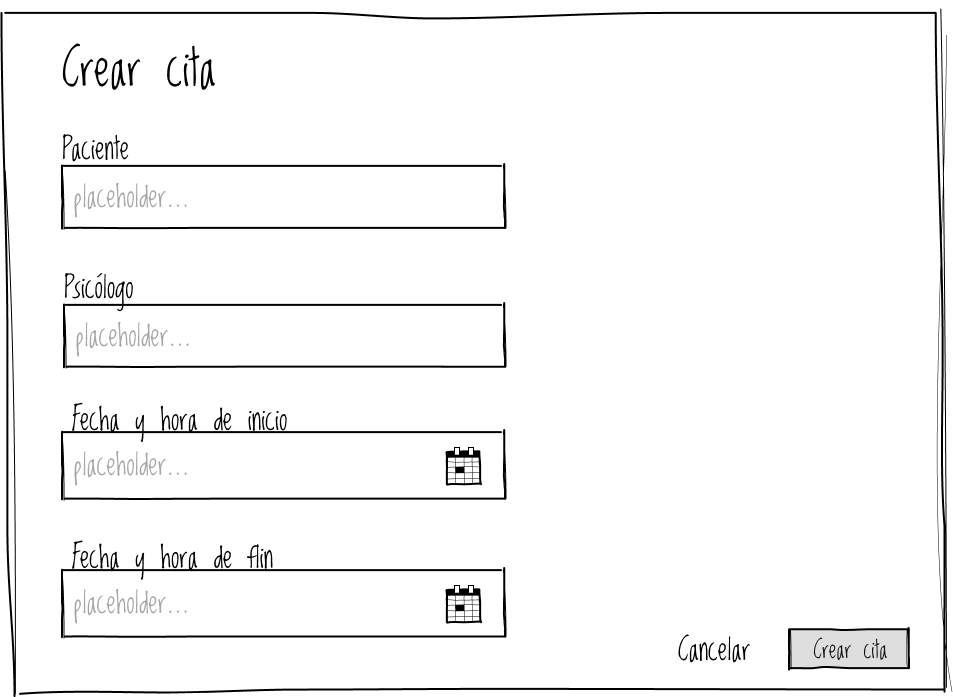
\includegraphics[scale=0.1]{doc/imagenes/dialogo-crear-cita.png}}
    \caption{Wireframe del diálogo de crear cita}
    \label{wireframe-crear-cita}
\end{figure}

\begin{figure}[H]
    \centering{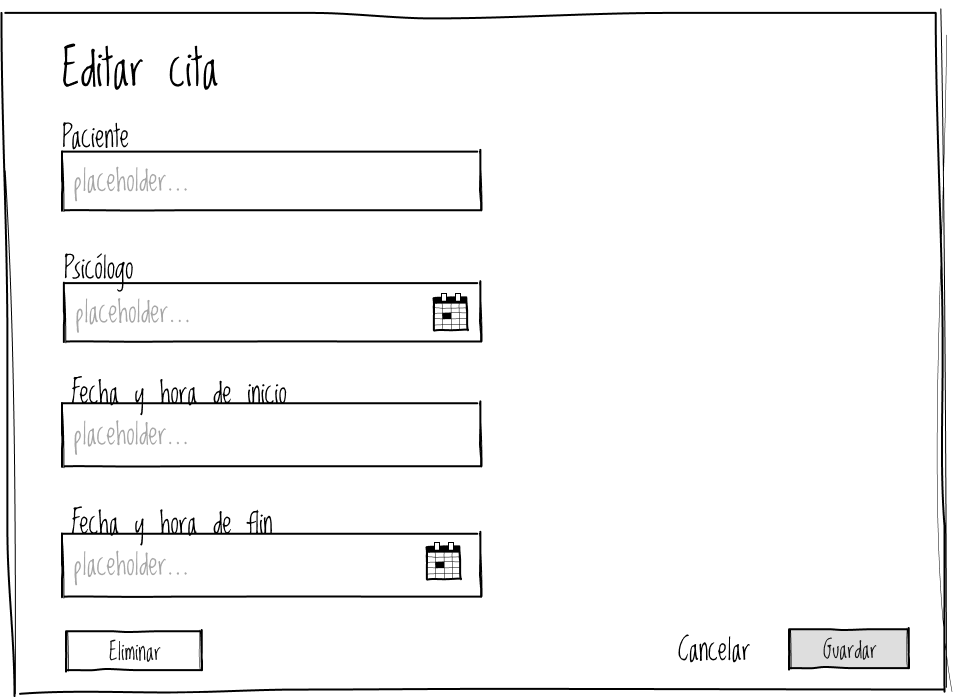
\includegraphics[scale=0.1]{doc/imagenes/dialogo-editar-cita.png}}
    \caption{Wireframe del diálogo de editar cita}
    \label{wireframe-editar-cita}
\end{figure}

Teniendo estos wireframes como guías para el diseño final de la plataforma, seguidamente se diseñaron los mockups en los que en algunos se hicieron algunas modificaciones en la estructura planteada en una primera instancia por los wireframes (Figuras \ref{mockup-login}, \ref{mockup-calendario}, \ref{mockup-menu} \ref{mockup-pacientes}, \ref{mockup-psicologos}, \ref{mockup-perfil}, \ref{mockup-add} y \ref{mockup-edit}). Sobretodo cabe mencionar que el menú lateral ha pasado a ser un desplegable. 

\begin{figure}[H]
    \centering{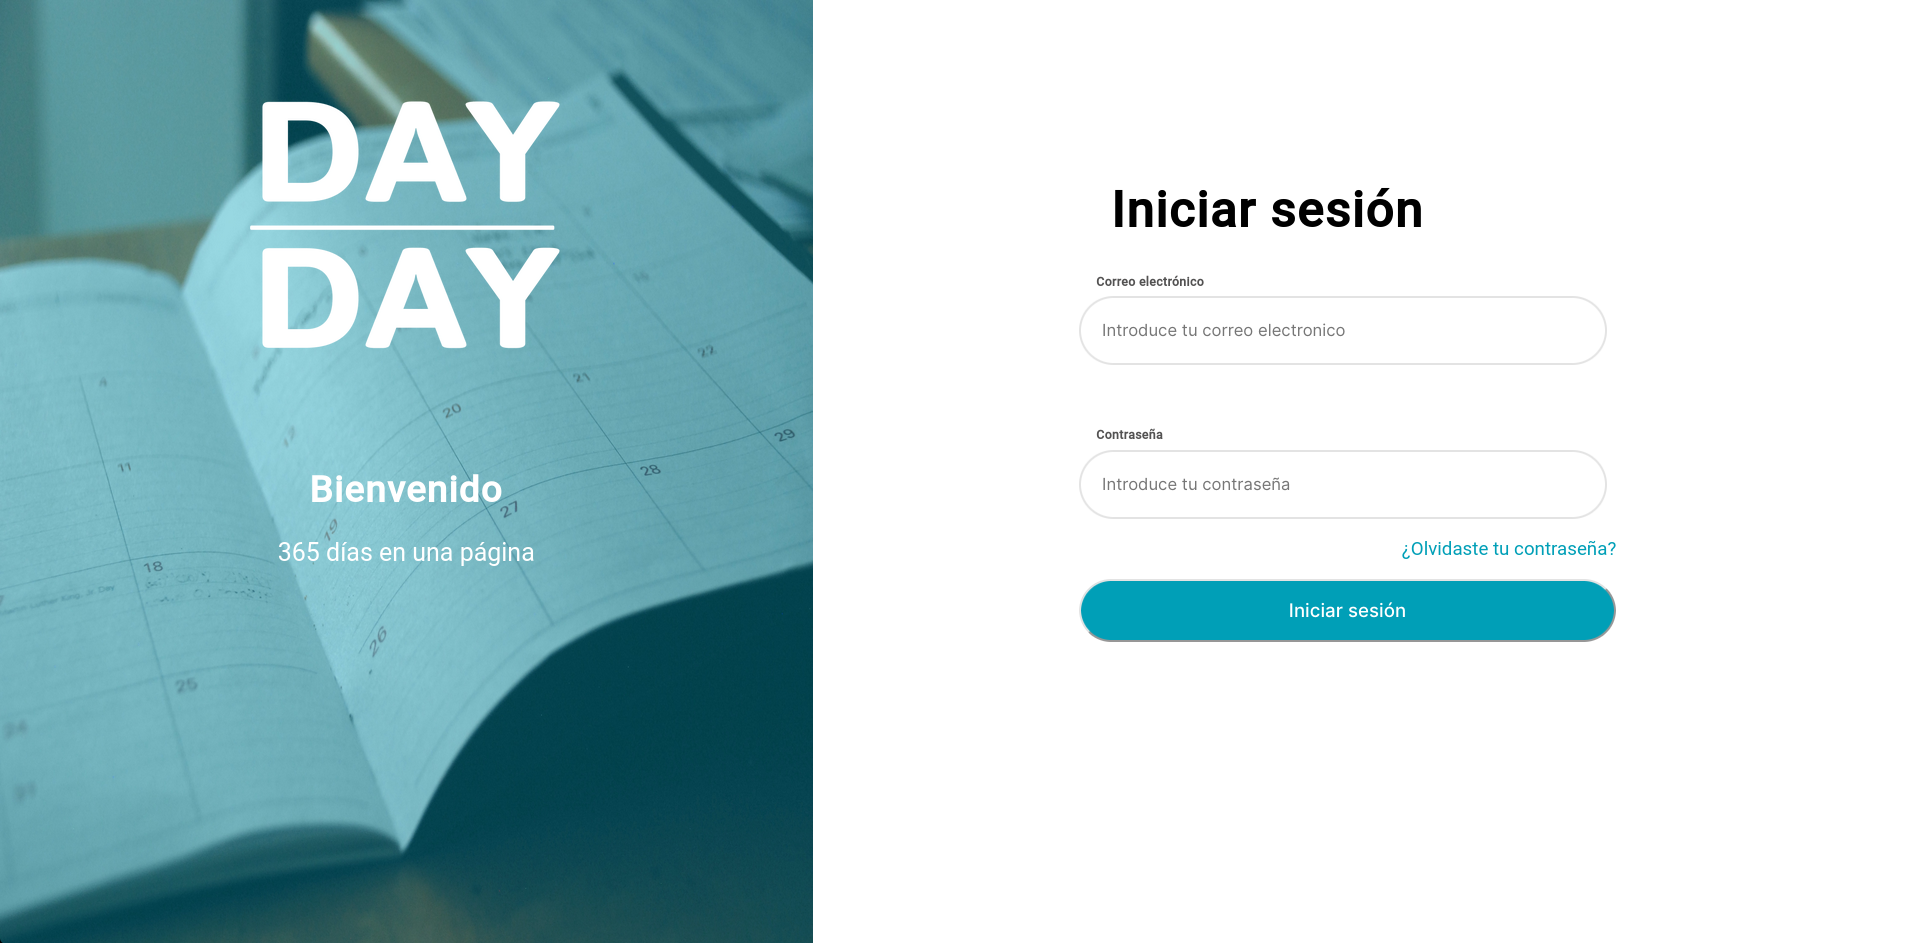
\includegraphics[scale=0.2]{doc/imagenes/mockup-login.png}}
    \caption{Mockup de la vista de Login}
    \label{mockup-login}
\end{figure}

\begin{figure}[H]
    \centering{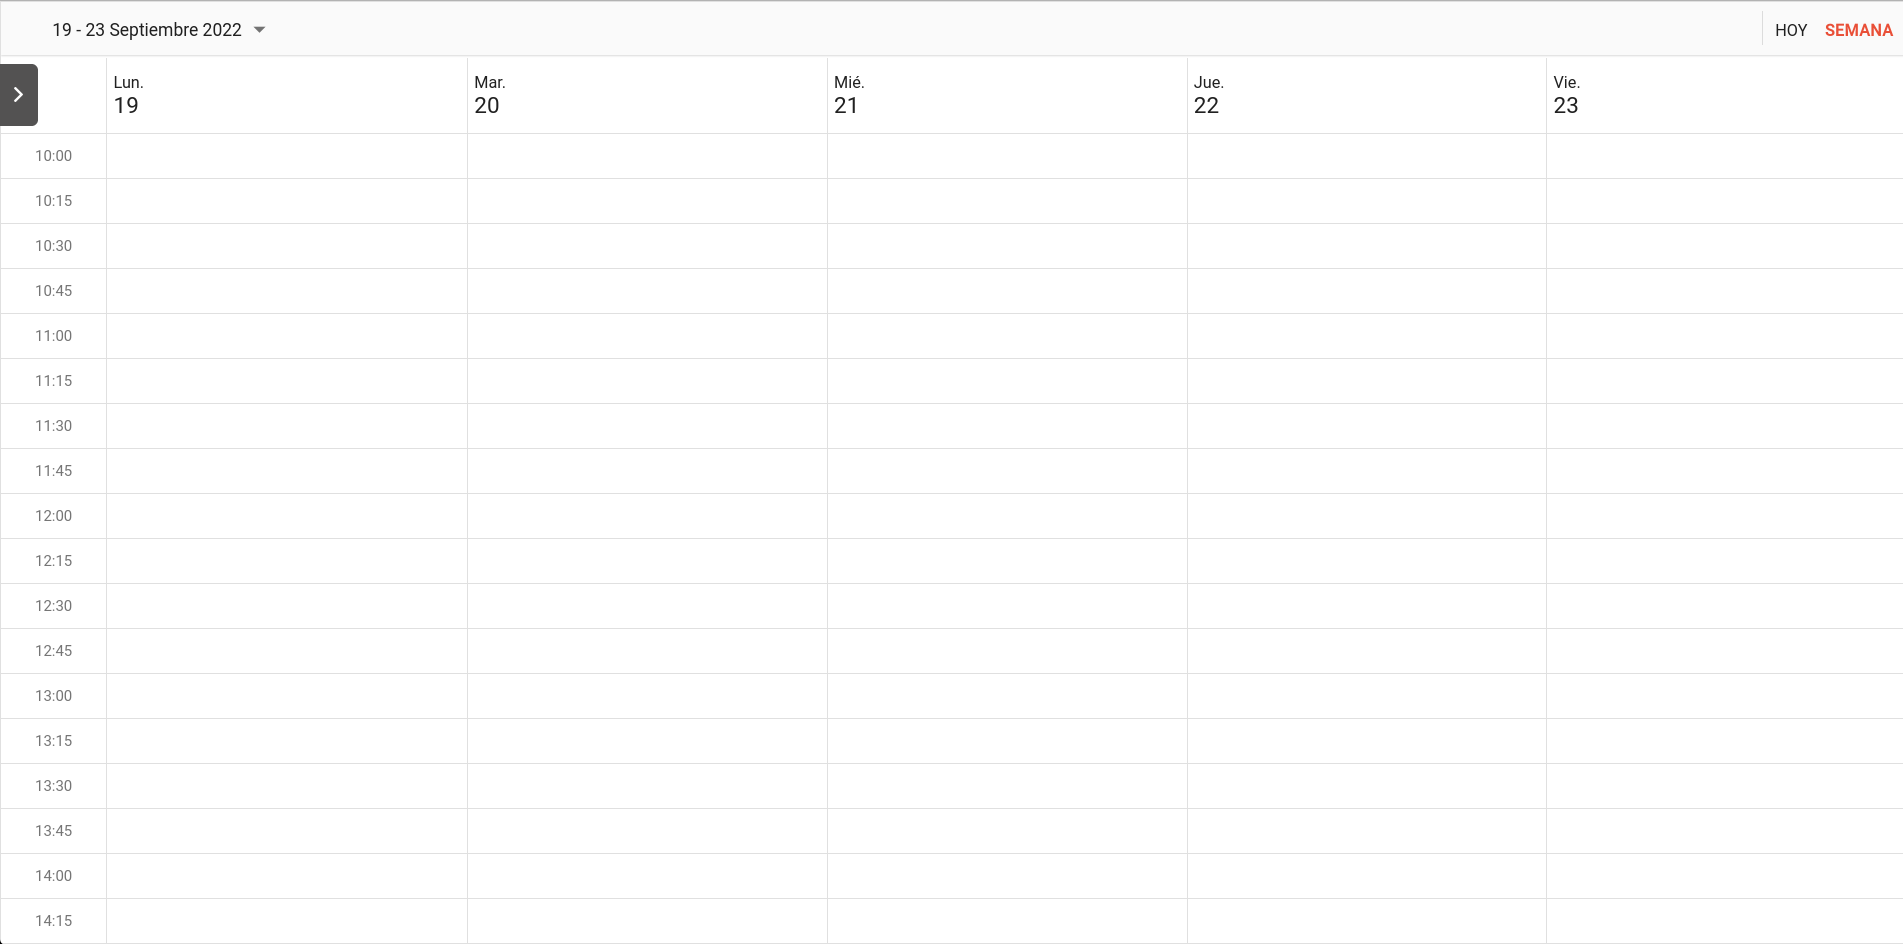
\includegraphics[scale=0.2]{doc/imagenes/mockup-calendario (1).png}}
    \caption{Mockup de la vista de Calendario}
    \label{mockup-calendario}
\end{figure}

\begin{figure}[H]
    \centering{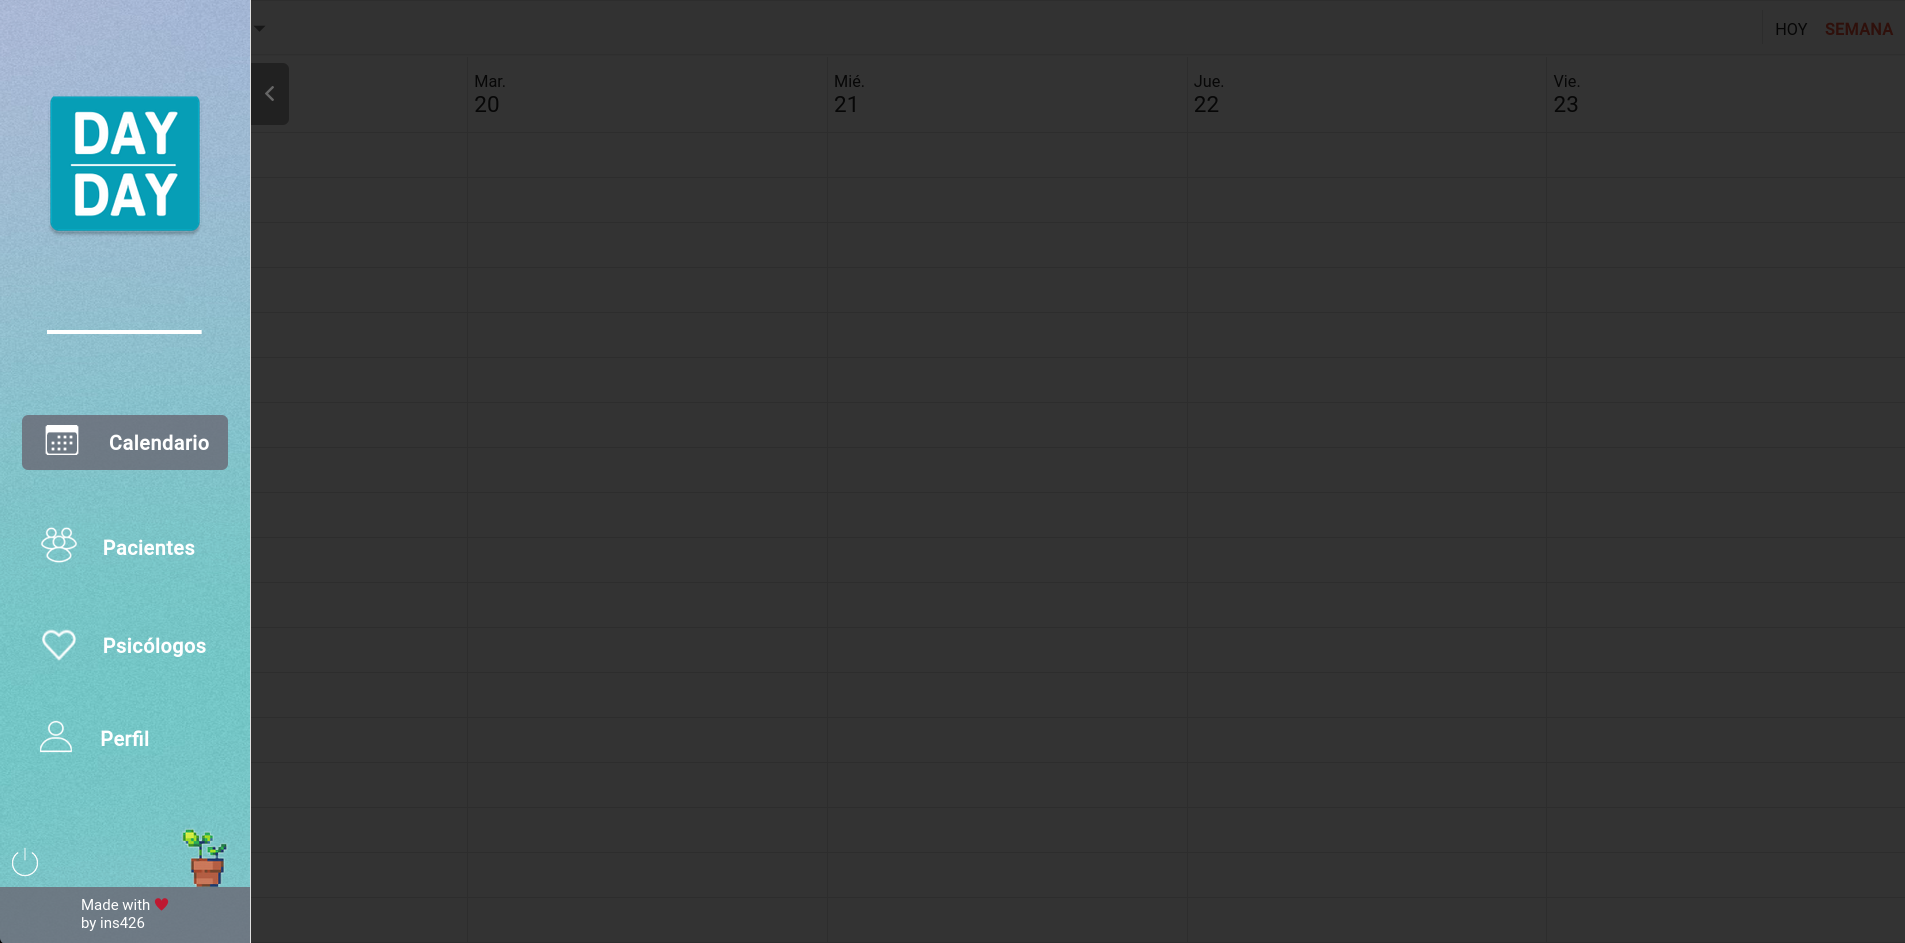
\includegraphics[scale=0.2]{doc/imagenes/mockup-menu.png}}
    \caption{Mockup de la vista de Calendario con el menú desplegado}
    \label{mockup-menu}
\end{figure}

\begin{figure}[H]
    \centering{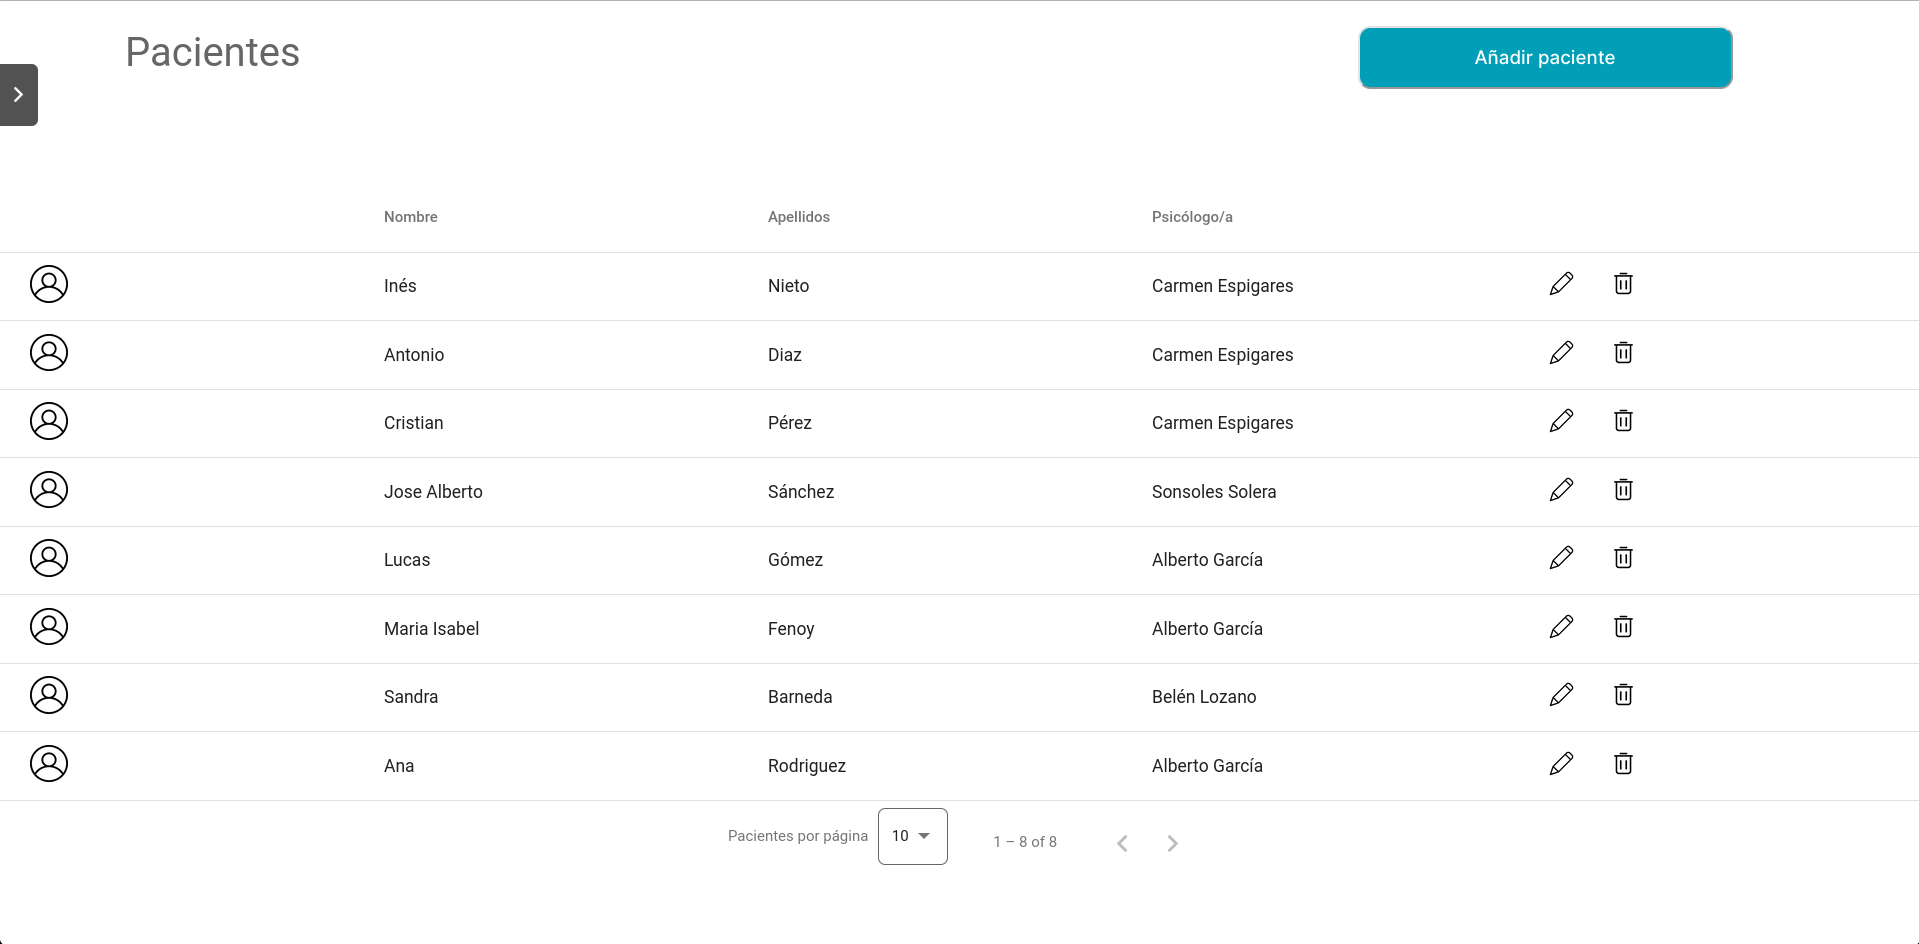
\includegraphics[scale=0.2]{doc/imagenes/mockup-pacientes.png}}
    \caption{Mockup de la vista de Pacientes}
    \label{mockup-pacientes}
\end{figure}

\begin{figure}[H]
    \centering{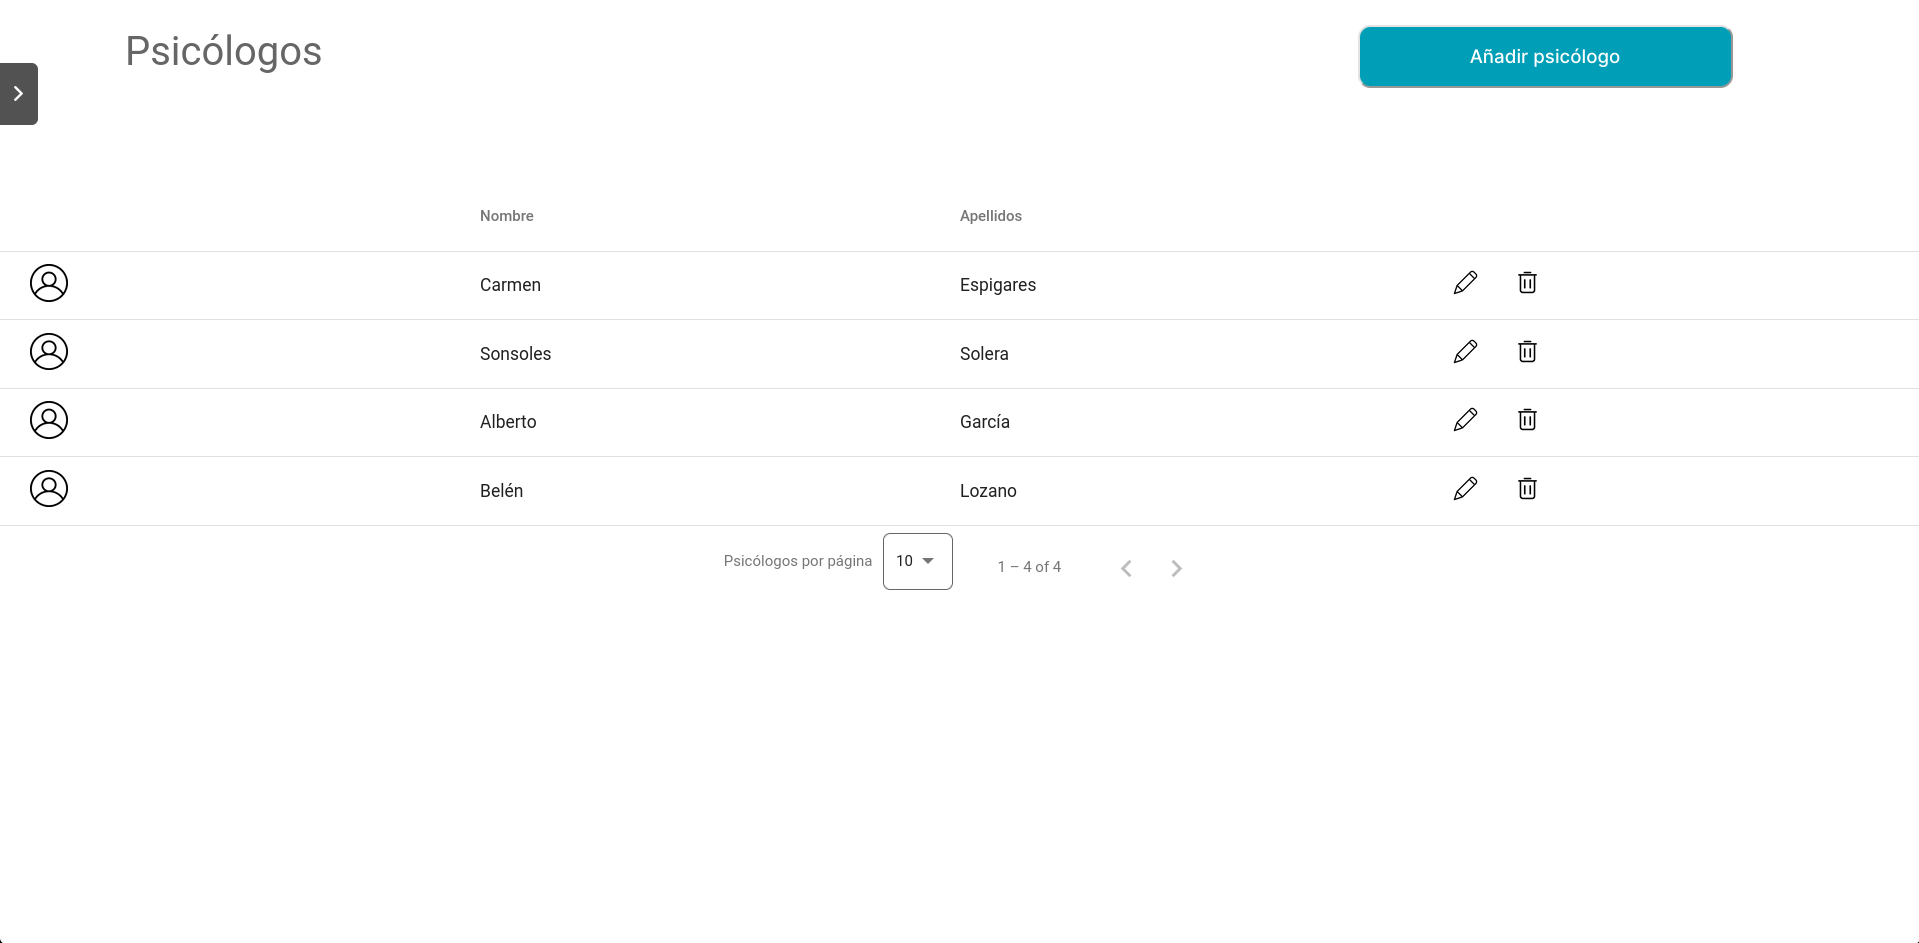
\includegraphics[scale=0.2]{doc/imagenes/mockup-psicologos.png}}
    \caption{Mockup de la vista de Psicólogos}
    \label{mockup-psicologos}
\end{figure}

\begin{figure}[H]
    \centering{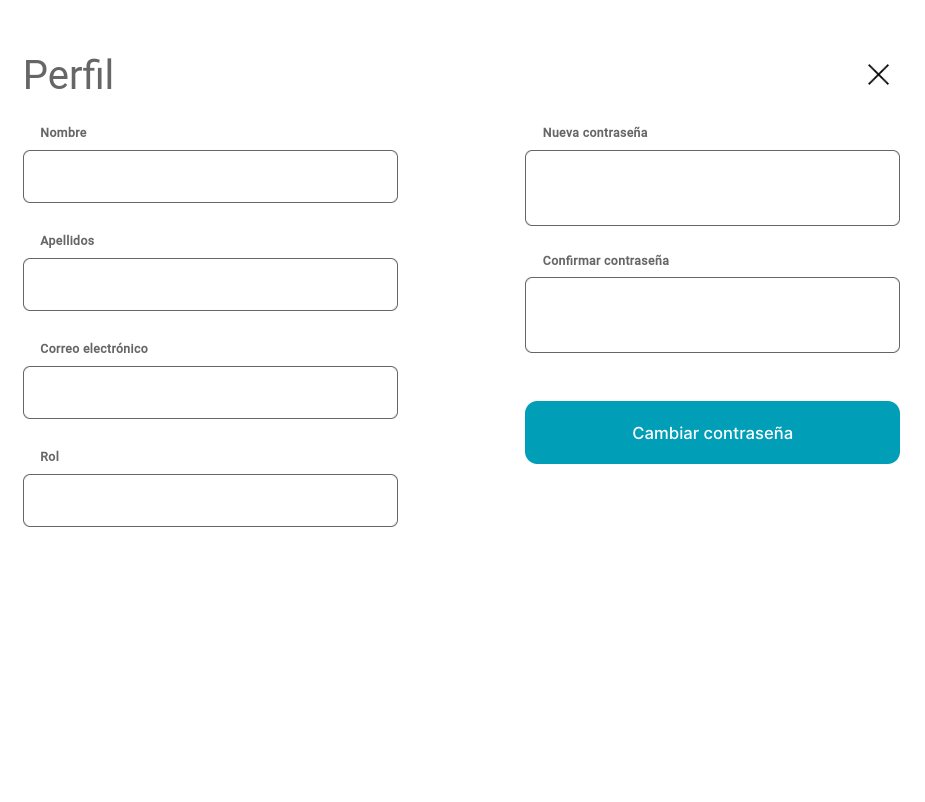
\includegraphics[scale=0.2]{doc/imagenes/mockup-perfil.png}}
    \caption{Mockup de la vista de Perfil}
    \label{mockup-perfil}
\end{figure}

\begin{figure}[H]
    \centering{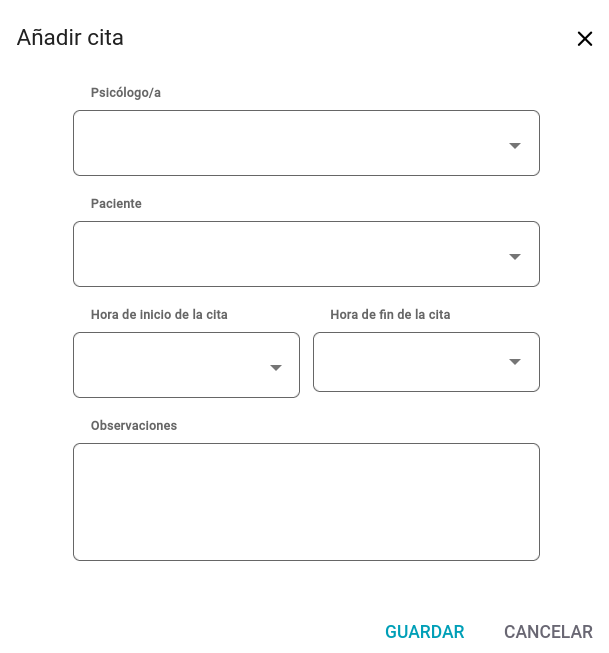
\includegraphics[scale=0.2]{doc/imagenes/mockup-add.png}}
    \caption{Mockup de la vista del diálogo de crear cita}
    \label{mockup-add}
\end{figure}

\begin{figure}[H]
    \centering{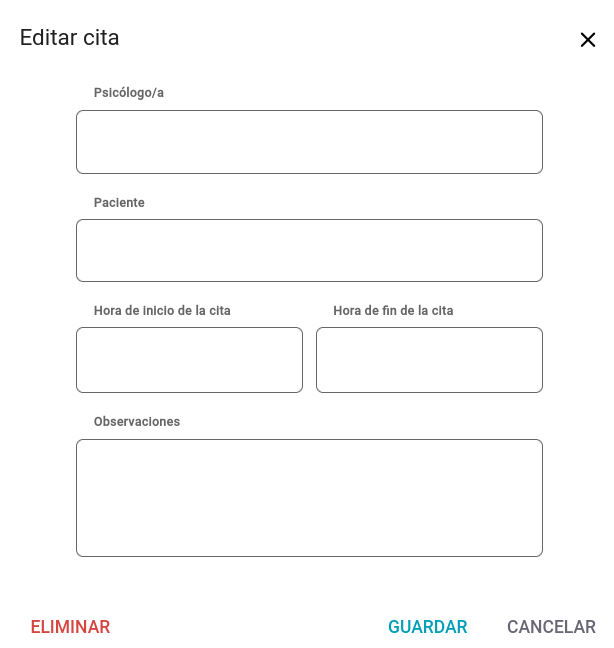
\includegraphics[scale=0.2]{doc/imagenes/mockup-edit.png}}
    \caption{Mockup de la vista del diálogo de editar cita}
    \label{mockup-edit}
\end{figure}
